\documentclass[11pt, a4paper,oneside,chapterprefix=false]{scrbook}

% setup with overleaf
\usepackage{a4wide}
\usepackage{times}
\usepackage{helvet}   % sets sans serif font

\usepackage{amsmath,amssymb,amsthm}
\usepackage{svg}
\usepackage{graphicx}
\usepackage{subfigure}  
\usepackage{fancybox} % for shadowed or double bordered boxes
\usepackage{fancyhdr}
\usepackage{float}
\usepackage{cite}
\usepackage{listings}
\usepackage{hyperref}
\usepackage{xargs}
\usepackage[colorinlistoftodos,prependcaption,textsize=tiny]{todonotes}


\newcommand{\todochange}[2][1=]{\todo[linecolor=blue,backgroundcolor=blue!25,bordercolor=blue,#1]{#2}}

\DeclareGraphicsExtensions{.pdf,.jpg,.png}

%% macros
 \def\mathbi#1{\textbf{\em #1}}
 
% commands
\newcommand{\Adjoint}{\mbox{\rm Adj}}
\newcommand{\Area}{\mbox{\rm Area}}
\newcommand{\ACos}{{\mbox{\rm Cos}^{-1}}}
\newcommand{\ASin}{{\mbox{\rm Sin}^{-1}}}
\newcommand{\ATan}{{\mbox{\rm atan2}}}
\newcommand{\Code}[1]{{\tt #1}}
\newcommand{\Complex}{\mbox{\bf C}}
\newcommand{\Cross}{{\mbox{\rm Cross}}}
\newcommand{\Mydddot}[1]{\mbox{\shortstack{$.$\hspace*{-1pt}$.$\hspace*{-1pt}$.$\\$#1$}}}
\newcommand{\Degree}{\mbox{\rm degree}}
\newcommand{\Diag}{\mbox{\rm Diag}}
\newcommand{\Dim}{\mbox{\rm dim}}
\newcommand{\Dist}{\mbox{\rm Distance}}
\newcommand{\IntTwo}{\int\!\!\int}
\newcommand{\IntThree}{\int\!\!\int\! \!\int}
\newcommand{\Kernel}{\mbox{\rm kernel}}
\newcommand{\Kross}{\mbox{\rm Kross}}
\newcommand{\Grad}{\nabla}
\newcommand{\Perp}{\mbox{\rm Perp}}
\newcommand{\Point}[1]{{\cal #1}}
\newcommand{\Rank}{\mbox{\rm rank}}
\newcommand{\Range}{\mbox{\rm range}}
\newcommand{\Real}{{\mbox{\rm I}\hspace*{-2pt}\mbox{\rm R}}}
\newcommand{\RealSbt}{{\mbox{\rm\scriptsize I}\hspace*{-2pt}\mbox{\rm\scriptsize R}}}
\newcommand{\Res}{\mbox{\rm resultant}}
\newcommand{\Sbt}[1]{{\mbox{\rm\scriptsize #1}}}
\newcommand{\MySign}{\mbox{\rm Sign}}
\newcommand{\SignSBT}{\mbox{\rm\scriptsize Sign}}
\newcommand{\Skew}{\mbox{\rm Skew}}
\newcommand{\Span}{\mbox{\rm Span}}
\newcommand{\SqrDist}{\mbox{\rm Distance$^2$}}
\newcommand{\Trace}{\mbox{\rm Trace}}
\newcommand{\TRN}{{\mbox{\rm\scriptsize T}}}
\newcommand{\Vector}[1]{\mbox{\bf #1}}
\newcommand{\VectorM}[1]{\mbox{\boldmath $#1$}}
\newcommand{\Volume}{\mbox{\rm Volume}}

\newcommand{\IVec}{\mbox{\boldmath $\imath$}}
\newcommand{\JVec}{\mbox{\boldmath $\jmath$}}
\newcommand{\KVec}{\mbox{\boldmath $k$}}
\newcommand{\LVec}{\mbox{\boldmath $\ell$}}
\newcommand{\RMat}{{\cal R}}
\newcommand{\QMat}{{\cal Q}}
\newcommand{\QCMat}{\overline{\cal Q}}

\newcommand{\Lerp}{\mbox{\rm lerp}}
\newcommand{\Slerp}{\mbox{\rm slerp}}
\newcommand{\Quad}{\mbox{\rm quad}}
\newcommand{\Squad}{\mbox{\rm squad}}

\newcommand{\ODer}[2]{\frac{d #1}{d #2}}
\newcommand{\ODerT}[2]{\frac{d^2 #1}{d {#2}^2}}
\newcommand{\ODerM}[3]{\frac{d #1}{d #2 \, d #3}}
\newcommand{\PDer}[2]{\frac{\partial #1}{\partial #2}}
\newcommand{\PDerT}[2]{\frac{\partial^2 #1}{\partial {#2}^2}}
\newcommand{\PDerM}[3]{\frac{\partial^2 #1}{\partial #2 \, \partial #3}}

% mass density symbol
\newcommand{\Den}{\delta}

% environments
\newenvironment{BArray}[1]{\left\{ \begin{array}{#1}}{\end{array} \right\}}
\newenvironment{Combin}{\left( \begin{array}{c}}{\end{array} \right)}
\newenvironment{Matrix}[1]{\left[ \begin{array}{#1}}{\end{array} \right]}


\let\mbf=\mathbf
\let\mvec=\mathbf
\let\mcal=\mathcal
\let\mfunc=\mathrm

%\def\R{\mbox{\ensuremath{\mathrm{I\!R}}}}
\newcommand{\R}{\ensuremath{\mathbb{R}}}
\newcommand{\N}{\ensuremath{\mathbb{N}}}
\newcommand{\Z}{\ensuremath{\mathbb{Z}}}
\newcommand{\C}{\ensuremath{\mathbb{C}}}

\newcommand{\of}[1]{\left( #1 \right)}
\newcommand{\abs}[1]{\left| #1 \right|}
\newcommand{\norm}[1]{\left\Vert {#1} \right\Vert}
\newcommand{\gradient}[1]{\nabla{\!}_{#1}{\,}}
\newcommand{\twovec}[2]{\left( #1 \atop #2 \right)}
\newcommand{\threevec}[3]{\left(\begin{array}{c}#1\\#2\\#3\end{array}\right)}
\newcommand{\fourvec}[4]{\left(\begin{array}{c}#1\\#2\\#3\\#4\end{array}\right)}

\newcommand{\refsec}[1]{Section~\ref{sec:#1}}
\newcommand{\reffig}[1]{Fig.~\ref{fig:#1}}
\newcommand{\reftab}[1]{Tab.~\ref{tab:#1}}
\newcommand{\refeq}[1]{Eq.~(\ref{eq:#1})}

%\newcommand{\R}{\hspace*{0.1ex}{\sf I} \hspace{-0.3ex}{\sf R}}

%6.5
\newcommand{\eps}{\mbox{$\epsilon$}}
\newcommand{\dmin}{\mbox{$d_{\min}$}}
\newcommand{\dmax}{\mbox{$d_{\max}$}}
\newcommand{\dminmax}{\mbox{$[\dmin,\dmax]$}}

%4.2:
\def\M{\mathcal{M}}
\def\n{\mathbi{n}}
\def\p{\mathbi{p}}
\def\q{\mathbi{q}}
\def\x{\mathbi{x}}
\def\tp{^{\mathsf{T}}}

\let\vec=\mathbi%
\let\mat=\mathbf%
\let\set= \mathcal%

% Taken from (and slightly modified): http://stackoverflow.com/questions/741985/latex-source-code-listing-like-in-professional-books

\usepackage{listings}
\usepackage{courier}
\usepackage{color}
\definecolor{lightgray}{gray}{0.9}
\definecolor{commentgreen}{rgb}{0.2,0.56,0.2}
 \lstset{
         basicstyle=\footnotesize\ttfamily, % Standardschrift
         numbers=left,               % Ort der Zeilennummern
         numberstyle=\tiny,          % Stil der Zeilennummern
         %stepnumber=2,               % Abstand zwischen den Zeilennummern
         numbersep=5pt,              % Abstand der Nummern zum Text
         tabsize=2,                  % Groesse von Tabs
         extendedchars=true,         %
         breaklines=true,            % Zeilen werden Umgebrochen
         keywordstyle=\color{red},
                frame=b,         
          keywordstyle=[1]\textbf,    % Stil der Keywords
         keywordstyle=[2]\textbf,    %
         keywordstyle=[3]\textbf,    %
         keywordstyle=[4]\textbf,   %\sqrt{\sqrt{}} %
         stringstyle=\color{blue}\ttfamily, % Farbe der String
         showspaces=false,           % Leerzeichen anzeigen ?
         showtabs=false,             % Tabs anzeigen ?
         xleftmargin=17pt,
         framexleftmargin=17pt,
         framexrightmargin=5pt,
         framexbottommargin=4pt,
         backgroundcolor=\color{lightgray},
         showstringspaces=false,      % Leerzeichen in Strings anzeigen ?
         commentstyle=\color{commentgreen}
 }
 \lstloadlanguages{% Check Dokumentation for further languages ...
         %[Visual]Basic
         %Pascal
         %C
		PHP, 
         C++
         %XML
         %HTML
         %Java
 }
    %\DeclareCaptionFont{blue}{\color{blue}} 

  %\captionsetup[lstlisting]{singlelinecheck=false, labelfont={blue}, textfont={blue}}
  \usepackage{caption}
\DeclareCaptionFont{white}{\color{white}}
\DeclareCaptionFormat{listing}{\colorbox[cmyk]{0.43, 0.35, 0.35,0.01}{\parbox{0.9972\textwidth}{\hspace{15pt}#1#2#3}}}
\captionsetup[lstlisting]{format=listing,labelfont=white,textfont=white, singlelinecheck=false, margin=0pt, font={bf,small}}

\usepackage{color}
\definecolor{RED}{rgb}{1,0,0}
\definecolor{GREEN}{rgb}{0,0.7,0}
\definecolor{BLUE}{rgb}{0,0,1}
\newcommand{\FIXME}[1]{{\color{RED}{\textbf{FIX}: #1}}}

\addtolength{\textheight}{2.0cm}
\addtolength{\voffset}{-1cm}
\addtolength{\textwidth}{1.8cm}
\addtolength{\hoffset}{-.9cm}

\widowpenalty=10000
\clubpenalty=10000

\lstdefinelanguage{json}{
    basicstyle=\normalfont\ttfamily,
    numbers=left,
    numberstyle=\scriptsize,
    stepnumber=1,
    numbersep=8pt,
    showstringspaces=false,
    breaklines=true,
    frame=lines,
    backgroundcolor=\color{background},
    stringstyle=\color{string},
    keywordstyle=\color{keyword},
    commentstyle=\color{comment},
    morecomment=[l]{//},
    morecomment=[s]{/*}{*/},
    morecomment=[l]{\#},
    morestring=[b]",
    morestring=[b]',
    morekeywords={true,false,null}
}

\definecolor{background}{HTML}{EEEEEE}
\definecolor{keyword}{RGB}{170,85,0}
\definecolor{string}{RGB}{0,128,0}
\definecolor{comment}{RGB}{128,128,128}

\lstdefinestyle{terminal}{
    backgroundcolor=\color{black},
    basicstyle=\ttfamily\color{white}\small,
    breaklines=true
}

\begin{document}

\frontmatter
%\maketitle %automatic version
% --- selfmade version ----
\begin{titlepage}
	\setlength{\parindent}{0cm}
	\addtolength{\textheight}{1.0cm}

	\vspace{0.2cm}
	\Huge
	\begin{center}
		{\textsf{\textbf{Analyzing the Impact of Occlusion on the Quality of Semantic Segmentation Methods for Point Cloud Data}}}	
	\end{center}
	

	\vfill \vfill \vfill
	\begin{figure}[h]
		\centering
		\includegraphics*[width=0.6\textwidth]{figures/titleimage_yf.png}
	\end{figure}

	\vfill
	\sffamily\Large
	\begin{center}
		{\textbf{Bachelor Thesis}} \\ 
		13th March 2023 - 13th September 2023 \\[0.5cm]
		\large
		Yufeng Xiao \\ 19-763-663
	\end{center}

	\vfill \vfill \vfill
	\begin{minipage}[b]{0.5\textwidth} \raggedright
	Supervisors: \\
	Prof. Dr. Renato Pajarola \\
	Lizeth Joseline Fuentes Perez \\
	\end{minipage}
	%
	\begin{minipage}[b]{0.5\textwidth} \raggedleft
	Visualization and MultiMedia Lab \\
	Department of Informatics \\
	University of Z{\"u}rich
	\end{minipage}

	\vfill
	\hrule
	\vspace{0.5cm}
	\includegraphics*[width=0.3\textwidth]{figures/uzh_logo} \hfill
	\includegraphics*[width=0.3\textwidth]{figures/vmml_logo}
\end{titlepage}
%%

%=====================================================================
\chapter{Abstract} \label{chp:abstract}
%=====================================================================

This work aims to analyze the impact of occlusion on the quality of semantic segmentation methods for point cloud data. Occlusion is a prevalent phenomenon in 3D scenes, where objects often overlap or obstruct each other. This can significantly compromise the quality and integrity of data, leading to inaccuracies in semantic segmentation. While the issue of occlusion has garnered attention in 3D data processing, current research on how different occlusion levels impact the quality of semantic segmentation is rare. Specifically, there's a palpable gap in understanding how to quantify occlusion in the scene and how this characteristic influence the performance of advanced semantic segmentation softwares like the Minkowski Engine. To bridge the research gap, we proposed a novel metric to quantify the occlusion level of a scene with viewpoint information. We then applied this metric to analyze the impact of occlusion on the quality of semantic segmentation methods for point cloud data. Our results show that the occlusion level of a scene is inversely proportional to the quality of semantic segmentation. This finding is crucial for advancing the state of the art in semantic segmentation and for paving the way for more robust applications in autonomous driving, robotics, and 3D scene analysis.

\tableofcontents

\mainmatter

%=====================================================================
\chapter{Introduction and Related Works} \label{chp:introduction}
%=====================================================================


Artificial intelligence has received significant attention in recent research. Fields such as natural language processing, image generation, and autonomous driving have benefited from considerable investments, and some related applications have been successfully implemented. Currently, the practical implementation of autonomous driving is still challenging due to the high demands for model performance and safety. To achieve its goals, AI needs to precisely understand its surrounding environment. Hence, semantic segmentation of scenes has become an essential topic. In this thesis, as opposed to focusing on outdoor scenes commonly associated with autonomous driving, we are more interested in understanding indoor environments. The correct classification and comprehension of indoor objects can assist in various aspects of human life, such as creating intelligent robots to help humans with a series of tasks. To understand scenes accurately, we need to provide AI with high-precision data, typically point clouds, which are a collection of data points defined in a three-dimensional coordinate system, represent the external surface of an object. These data points can capture the shape, and sometimes color, of the physical entities in a scanned environment. They are usually obtained from laser scanners or multi-view reconstructions. However, when collecting this type of data, objects are often obstructed due to the viewpoint of the scanner, leading to occlusions in the data, as shown in Figure \ref{fig:occlusion in a scene} [S3dis], where part of occlusions in a scene are marked with red box. Therefore, we aim to explore how occlusion affects AI's understanding of a scene. More specifically, we want to propose a metric to reflect the occlusion level of a scene and analyze how this characteristic influences the performance of semantic segmentation methods.

% \todo{Describe the input point cloud characteristics and the expected output (occlussion metric)}
% \todo{ii) Why is this metric important}
% \todo{ applications where occlusion can be potentially used (semantic segmentation)}

\begin{figure}[h]
    \centering
    \includegraphics*[width=0.8\textwidth]{figures/occlusion in conf2.png}
    \caption{Occlusion in a scene}
    \label{fig:occlusion in a scene}
\end{figure}

\section{Previous work}
To the best of our knowledge currently there is not explicit works that compute occlusion level for an entire indoor scene. There are some related works handling occlusion of point cloud. In this section, we will briefly introduce these works, especially the ones that are related to occlusion.  

% \todo{ briefly mention related works that use occlusion}
% \todo{ summarize the occlusion part in this papers}

\paragraph{Occlusion Guided Scene Flow Estimation on 3D Point Clouds.}

This paper presents the OGSF-Net, a novel architecture designed to address the challenges of occlusions in 3D scene flow estimation. Occlusions, where certain regions in one frame are hidden in another, can hinder accurate flow estimation. The OGSF-Net uniquely integrates the learning of flow and occlusions, using an occlusion handling mechanism in its Cost Volume layer to measure frame correlations. This approach aims to enhance both flow accuracy and the understanding of occluded regions, marking a pioneering effort in 3D scene flow estimation on point clouds. To make this method robust, it's important to make an accurate occlusion prediction. Therefore, they evaluate the performance of occlusion estimation on dataset FlyingThings3D, which provides the ground truth occlusion mask of point cloud. For evaluation, they use accuracy and F1 score as metrics. This inspires us to apply similar metrics to evaluate the result of semantic segmentation.

\paragraph{OcCo: Unsupervised Point Cloud Pre-training via Occlusion Completion.} \label{par:occlusion completion}

In this work, the authors proposed ${Occlusion Completion}$, an unsupervised pre-training method. The main idea is to generate occlusion in a point cloud, then use an encoder-decoder model to reconstruct occluded points, and apply the encoder weighths for downstream tasks. What is interesting for us is how they generate occlusion in a scene. They view point cloud from a camera, which is placed in different viewpoints. At each viewpoint, points are projected to a camera reference frame, if some points share the same pixel coordinates, then there might be occlusion. This could also be an inspiration for us to generate occlusion in a scene.

\section{Positioning and Contributions}

Previous work has shown that occluison of a point cloud can be estimated based on ground truth occlusion information. However, in our work we have to estimate occlusion level of a scene without knowing such information. To achieve this, we decide to create occlusion in the scene by placing viewpoints in different locations. With the dataset we created, we can propose a metric to quantify the occlusion level of a scene. If we think about occlusion level of a scene in real world, our intuition is that the more viewpoints we use to look at a scene, the more area of the scene we can see. Therefore, we propose a metric that is based on the ratio between visible area and total area of the scene. Since there's no surface area information in a point cloud, we would first validate our metric on mesh. To extend the concept ${Visible Area Ratio}$ to point cloud, we would use ${Occlusion Ray}$, which means the ray hit occlusion in the scene, to estimate occlusion level.

% Observations: Previous work knows the GT occlussion information and computes the oclusion level with a conventional metric F1 score. 
% Defined as classification (formal definition).

% \todo{Solution: Our insights and technical contributions are:}
% Metric 
% We validate our results by creating a dataset with occlusion.
% We are the first one to define oclusion in a scene without viewpoint information.
% How do you define the metric?
% Ratio between visible area and total area of the scene.
% How do we compute area in a triangular mesh?
% How do we extend this to a point cloud scenario?

%=====================================================================
\section{Technical Background}
%=====================================================================

Based on the introduction in previous sections, we would elaborate on some key concepts in the technical background of this work.

\subsection{Point Cloud Data}

A point cloud is a discrete set of data points in space. The points may represent a 3D shape or object. Each point position has its set of Cartesian coordinates (X, Y, Z), in some cases it can also include color(RGB) or intensity information. Point clouds are generally produced by 3D scanners or by photogrammetry software, which measure many points on the external surfaces of objects around them.[wiki] 

\vspace{10pt}

Point cloud can be used in different areas. One usage is for rendering and modeling. Typically 3D objects are modeled using polygon meshes, and  polygons are the rendering primitives in the graphics pipeline. However, representing all objects with point sampling allows easy mixing of objects in a scene without specialized algorithms for different geometry types. Other applications include depth sensing, perception, scientific computing etc.

\subsection{Semantic Segmentation}

Semantic segmentation for point cloud data has rapidly ascended as a pivotal research domain, given its profound implications in a myriad of applications. From the intricate pathways navigated by autonomous vehicles to the precise movements of robotics and the detailed analysis of 3D scenes, the ability to accurately segment and categorize each data point in a 3D environment is important.

\vspace{10pt}

At the heart of this research lies the challenge of dealing with occlusions. In real-world scenarios, objects within a scene often overlap or obstruct each other, leading to partial or even complete occlusions. Such occlusions can significantly distort the spatial distribution of data points, making it challenging to discern the true structure and category of the obstructed objects. For instance, in an urban driving scenario, a pedestrian might be partially hidden behind a parked car, or in an indoor setting, a chair might be obscured by a table. These occlusions can lead to misclassifications, reducing the overall accuracy of the segmentation process.

\vspace{10pt}

This project proposal is rooted in the quest to unravel the intricacies of occlusion within point cloud data. Specifically, we aim to delve deep into understanding how varying levels of occlusion in a scene impact the performance and quality of semantic segmentation methods. By systematically analyzing the effects of occlusion, we aspire to shed light on potential strategies to enhance segmentation accuracy, even in highly occluded environments.

\paragraph{Minkowski Engine.}

The Minkowski Engine stands out as a state-of-the-art tool in this domain. It is an auto-differentiation library specifically designed for sparse tensors. In the area of deep learning, where dense tensors are commonly used, the Minkowski Engine brings a fresh perspective by focusing on sparse tensors. This is particularly beneficial for 3D data, which often exhibits spatial sparsity. The engine supports all standard neural network layers, including convolution, pooling, unpooling, and broadcasting operations, but tailored for sparse tensors. Such capabilities make it an ideal choice for semantic segmentation tasks, especially when dealing with point cloud data.

\begin{figure}[h]
    \centering
    \includegraphics*[width=0.8\textwidth]{figures/Minkowski Engine.png}
    \caption{Minkowski Engine Indoor Scene Segmentation}
    \label{fig:minkowski}
\end{figure}


\section{Motivation} \label{sec:motivation}

Among the myriad factors influencing the semantic segmentation of point cloud data, the level of occlusion stands as a paramount challenge. Occlusions, a prevalent phenomenon in 3D scenes, can significantly compromise the quality and integrity of data. When objects are partially or entirely obscured by others, conventional semantic segmentation approaches might falter, leading to inaccuracies in segmentation. While the issue of occlusion has garnered attention in 3D data processing, current research on how different occlusion levels impact the quality of semantic segmentation remains fragmented. Specifically, there's a palpable gap in understanding how to quantify occlusion levels and how these levels influence the performance of advanced tools like the Minkowski Engine. 

\vspace{10pt}

Thus, the primary motivation behind this research is to systematically evaluate occlusion levels and delve deep into their implications on point cloud data semantic segmentation. Through this investigation, we aim to offer more precise semantic segmentation methodologies, especially in environments with high levels of occlusion. In essence, our objective is to forge a nexus between occlusion levels and the efficacy of semantic segmentation, providing invaluable insights for future research and applications.

\section{Outline} \label{sec:outline}

In this work we use ray-tracing based methods to scan ground truth cloud and compute occlusion level for the scanned cloud. Before we doing this, we apply similar methods to estimate occlusion level of mesh to validate that ray-based methods are reliable. Finally, an interactive web application is developed to visualize the point cloud together with a backend is developed to compute the occlusion level of the point cloud.


%=====================================================================
\chapter{Problem Statement} \label{chp:problem}
%=====================================================================



\section{Occlusion Level Computation of Mesh} \label{sec:occlusion}

We have to validate here that more viewpoints lead to lower occlusion level of the interior scene.

\begin{figure}[htp]
	\centering
	\subfigure[1 viewpoint]{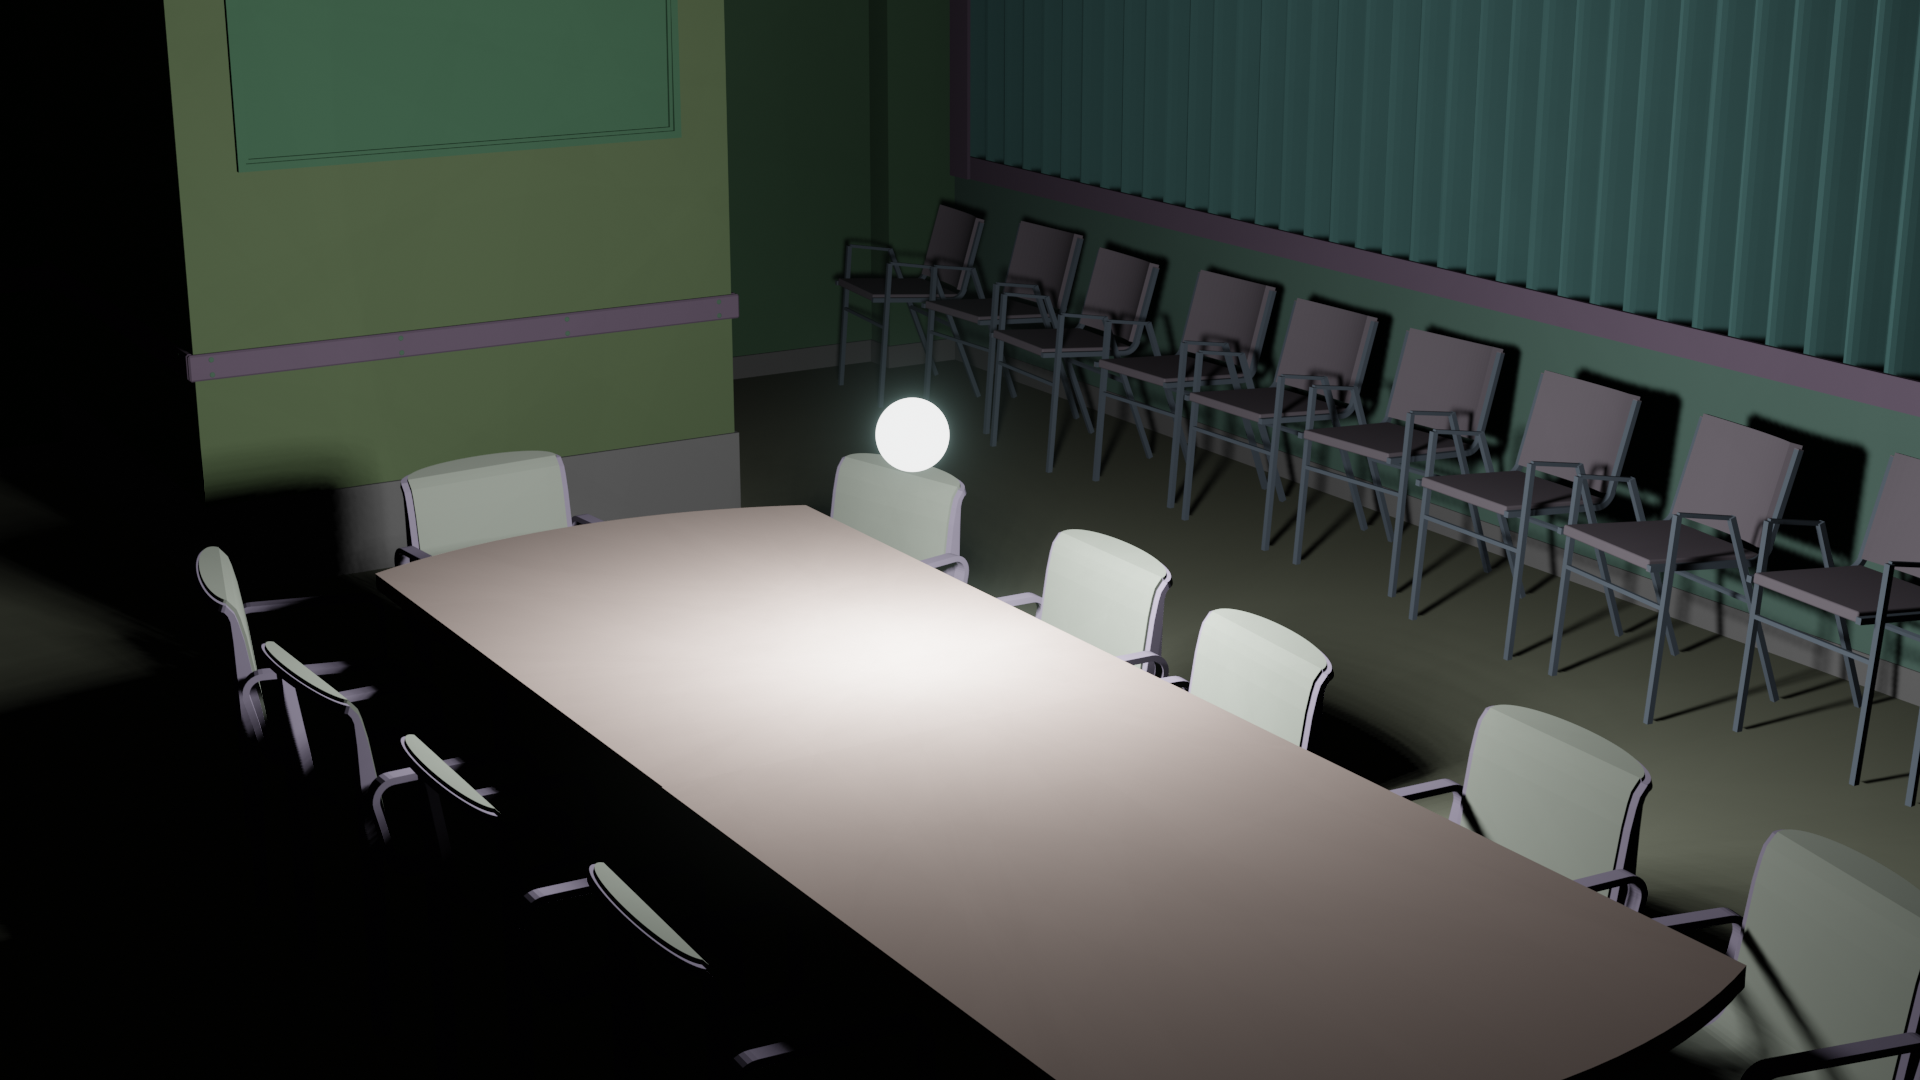
\includegraphics[width=0.45\textwidth]{figures/1 vp.png} \label{fig:1 vp}} \hfill
	\subfigure[2 viewpoints]{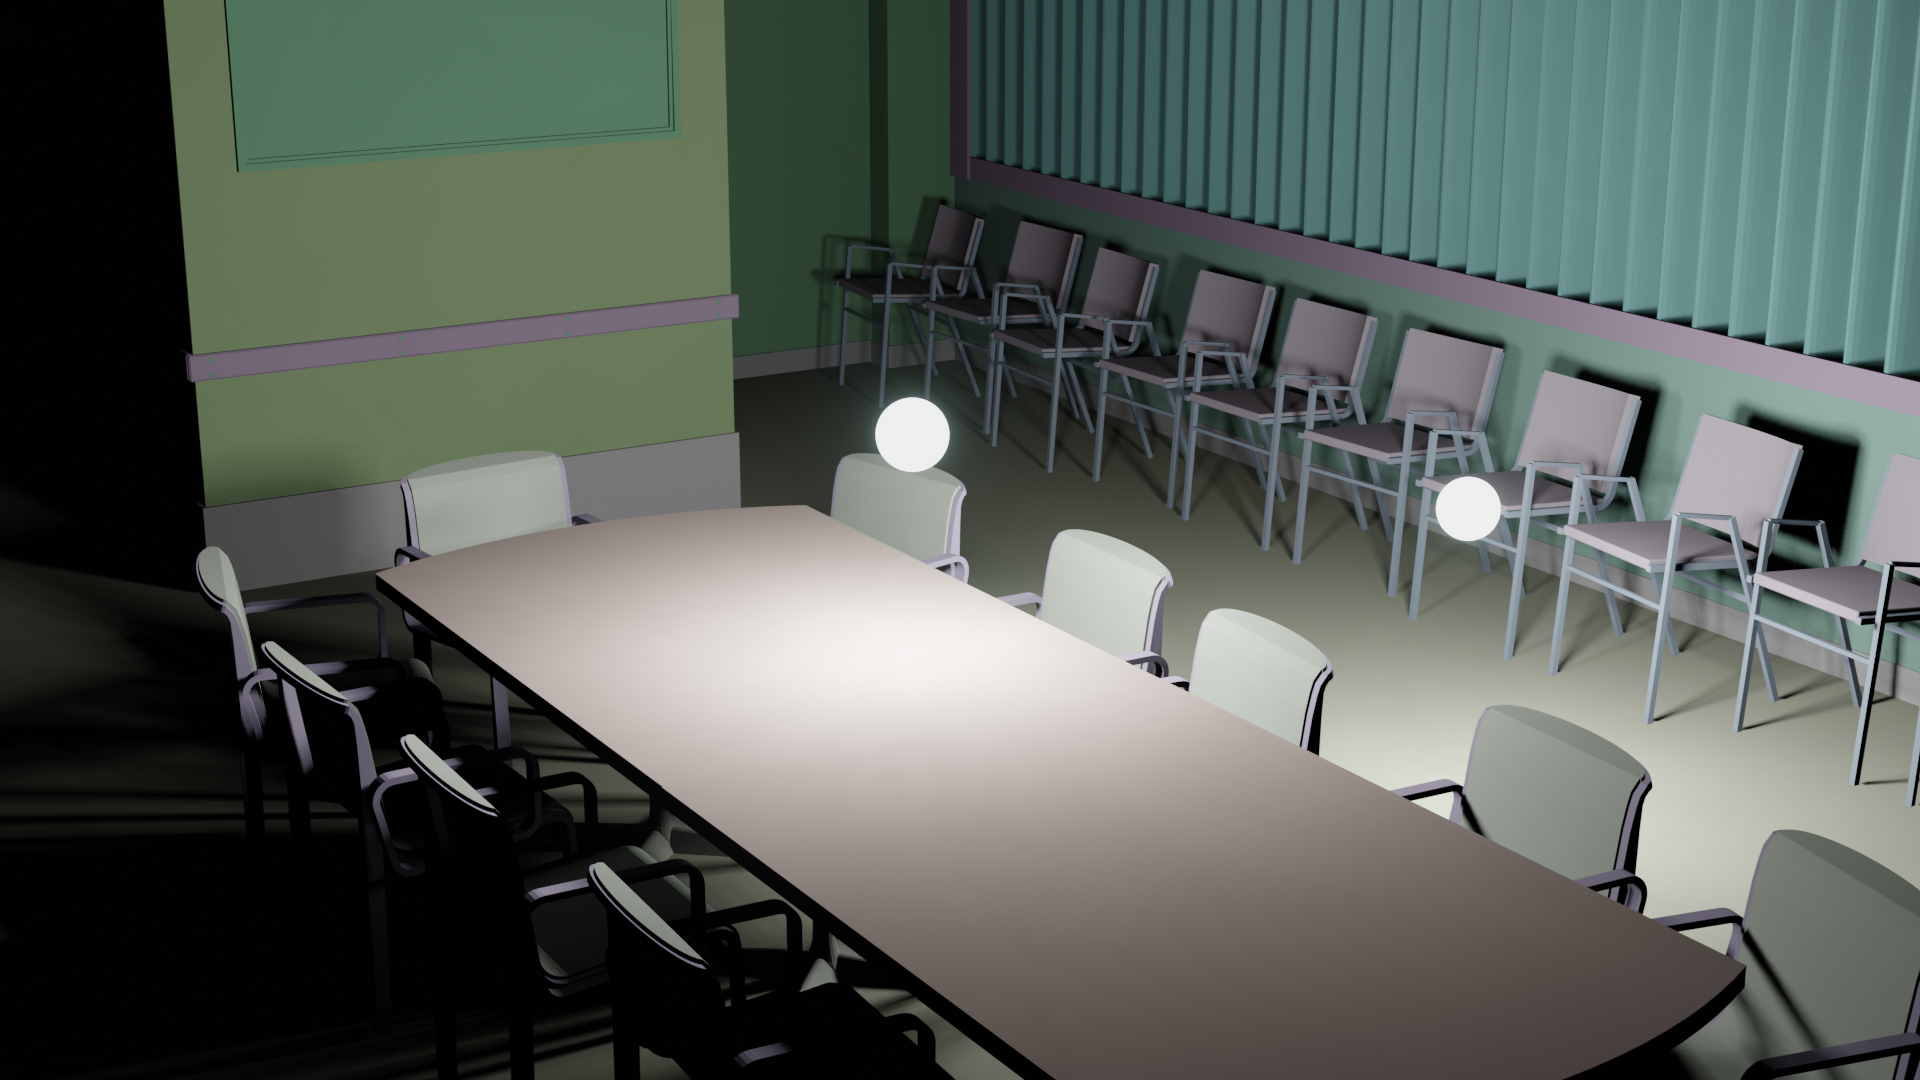
\includegraphics[width=0.45\textwidth]{figures/2 vp.png} \label{fig:2 vp}}
	\caption{Scene with Light Sources}
	\label{fig:scene with light sources}
\end{figure}


\subsection{Ground Truth Mesh} \label{subsec:occlusion}

We should compute the occlusion level of ground truth mesh.

\subsection{Estimated Mesh from Point Cloud} \label{subsec:occlusion}

We also want to estimate the occlusion level of the mesh generated from ground truth point cloud.
\todo{Why do we wanna do this?}

\section{Occlusion Level Computation of Point Cloud} \label{sec:occlusion}

After validation in previous steps, we should directly compute the occlusion level of the ground truth point cloud.

\section{Evaluation of Segmentation Result} \label{sec:evaluation}

It's essential to evaluate result of segmentation of point cloud so that we can maybe find correlation between occlusion level and segmentation performance.

%=====================================================================
\chapter{Technical Solution} \label{chp:solution}
%=====================================================================

In this chapter we will introduce our technical solution to the problem stated in \ref{chp:problem}.

\section{Ray Tracing Based Estimation of Visible Area Ratio} \label{sec:ray tracing visible area ratio}

Ray tracing is a powerful technique used in computer graphics to simulate the way light interacts with objects to generate realistic images. In the context of our study, ray tracing plays a pivotal role in estimating the visible area ratio of triangles in a scene. This estimation is crucial for understanding how much of a triangle's surface is directly illuminated by a light source, especially when other objects in the scene might occlude it.

\vspace{10pt}

A flow chart of the whole pipeline is shown here.

\begin{minipage}{\textwidth}
	\begin{figure}[H]
		\centering
		\includegraphics*[width=1.0\textwidth]{figures/visible area.png}
		\caption{Flow chart of visible area ratio estimation}
		\label{fig:visible area ratio estimation}
	\end{figure}
\end{minipage}

\subsection{Uniform Sample Triangles}

To accurately represent a triangle's area using samplings, it's imperative that these samplings comprehensively cover the triangle. For this purpose, we employ the random uniform sampling method. This method ensures that each point within the triangle has an equal chance of being selected, leading to a fair representation of the triangle's entire area.

\vspace{10pt}

The process begins by randomly generating two parameters, \( r_1 \) and \( r_2 \), both of which lie in the interval [0, 1]. These random parameters are then used to compute the barycentric coordinates of the sampled points within the triangle. The barycentric coordinates, denoted as \( \alpha \), \( \beta \), and \( \gamma \), allow us to express any point within the triangle as a linear combination of the triangle's vertices.

\vspace{10pt}

To derive the sampled point's coordinates using \( r_1 \) and \( r_2 \), we use the following equations:
\[ \alpha = 1 - \sqrt{r_1} \]
\[ \beta = \sqrt{r_1} \times r_2 \]
\[ \gamma = 1 - \alpha - \beta \]
\[ P = \alpha V_1 + \beta V_2 + \gamma V_3 \]

Where \( P \) is the sampled point, and \( V_1 \), \( V_2 \), and \( V_3 \) are the triangle's vertices. Below is a visualization of the uniform sampling method.

\begin{minipage}{\textwidth}
	\begin{figure}[H]
		\centering
		\includegraphics*[width=0.6\textwidth]{figures/uniform sample triangle.png}
		\caption{Uniform Sample Triangle}
		\label{fig:uniform sample triangle}
	\end{figure}
\end{minipage}

\subsection{Generate Rays}

In computer graphics, especially in the context of ray tracing, generating rays is a fundamental step. These rays simulate the path of light as it interacts with objects in a scene. In our approach, we generate rays from the sampled points on the triangle to a light source. This is crucial for determining how light interacts with the triangle, especially when considering factors like shading and occlusion.

\vspace{10pt}

The sampled points serve as the origin of each ray, while the view point (or light source) acts as the look-at point. The direction of each ray is computed based on the difference between the look-at point and the origin. The direction vector is then normalized to ensure its magnitude is 1, which simplifies subsequent calculations.

\vspace{10pt}

The direction of the ray, \( \text{Direction} \), can be computed as:

\begin{equation}
	\text{Direction} = \frac{\text{LookAt} - \text{Origin}}{\|\text{LookAt} - \text{Origin}\|}
\end{equation}

Where:
\begin{itemize}
    \item \(\text{Origin}\) is the starting point of the ray, which in our case is the sampled point on the triangle.
    \item \(\text{Destination}\) is the end point of the ray, typically representing the viewpoint or light source.
\end{itemize}

By generating rays in this manner, we can accurately simulate the behavior of light as it travels from the triangle to the viewpoint or light source. This is essential for producing realistic renderings and for analyzing the effects of various factors, such as occlusion, on the final image.


\subsection{Ray Triangle Intersection}

Ray-triangle intersection is a fundamental operation in computer graphics, especially in the context of ray tracing. Determining whether a ray intersects a triangle and finding the intersection point are crucial for rendering scenes composed of triangular meshes.

\vspace{10pt}

One of the most efficient and widely used algorithms for this purpose is the Möller–Trumbore intersection algorithm. This algorithm determines the intersection of a ray and a triangle in a 3D space without any need for pre-computed plane equations.

\vspace{10pt}

Given a ray represented by its origin \( O \) and direction \( D \), and a triangle defined by its vertices \( V_1 \), \( V_2 \), and \( V_3 \), the algorithm computes the intersection using barycentric coordinates.

\vspace{10pt}

The intersection point \( P \) can be represented as:
\[ P = (1 - u - v) V_1 + u V_2 + v V_3 \]

Where \( u \) and \( v \) are the barycentric coordinates. The ray intersects the triangle if \( 0 \leq u \leq 1 \), \( 0 \leq v \leq 1 \), and \( u + v \leq 1 \).

\begin{minipage}{\textwidth}
	\begin{figure}[H]
		\centering
		\includegraphics*[width=0.25\textwidth]{figures/intersect polygon.png}
		\caption{Ray Intersect Triangle}
		\label{fig:ray intersect triangle}
	\end{figure}
\end{minipage}

The algorithm uses the following equations to compute \( u \), \( v \), and \( t \) (where \( t \) is the distance from the ray origin to the intersection point):

\begin{itemize}
    \item \textbf{Edge Vectors:} These vectors represent two edges of the triangle.
	\[ e_1 = V_2 - V_1 \]
	\[ e_2 = V_3 - V_1 \]
	
    \item \textbf{Vector \( h \):} The cross product of the ray direction and \( e_2 \).
    \[ h = D \times e_2 \]
    
    \item \textbf{Determinant \( a \):} It's used to check if the ray is nearly parallel to the triangle.
    \[ a = e_1 \cdot h \]
    
    \item \textbf{Factor \( f \):} Used for subsequent calculations.
    \[ f = \frac{1}{a} \]
    
    \item \textbf{Vector \( s \):} Represents the vector from the ray's origin to one vertex of the triangle.
    \[ s = O - V_1 \]
    
    \item \textbf{Barycentric Coordinate \( u \):} The first computed barycentric coordinate.
    \[ u = f (s \cdot h) \]
    
    \item \textbf{Vector \( q \):} The cross product of vector \( s \) and \( e_1 \).
    \[ q = s \times e_1 \]
    
    \item \textbf{Barycentric Coordinate \( v \):} The second computed barycentric coordinate.
    \[ v = f (D \cdot q) \]
    
    \item \textbf{Distance \( t \) to Intersection:} Represents the distance from the ray's origin to the intersection point.
    \[ t = f (e_2 \cdot q) \]
\end{itemize}

The algorithm first checks if \( a \) is close to zero, which means the ray is nearly parallel to the triangle and thus, likely does not intersect it. If \( a \) is not close to zero, the algorithm proceeds to compute \( u \), \( v \), and \( t \) to determine the intersection.

This algorithm is both efficient and robust, making it a popular choice for ray-triangle intersection tests in various graphics applications.

\subsection{Visible Area Ratio}

In the context of ray tracing and light interaction, understanding the visible area of a triangle is crucial. The visible area ratio provides insight into how much of a triangle's surface is directly illuminated by a light source without being occluded by other objects in the scene.

\vspace{10pt}

From the previous steps, we have computed samplings on each triangle and generated rays originating from these samplings directed towards the light source. To determine the visible area, we first need to compute the visibility weight for each sampling. This weight represents the ratio of visible samplings to the total number of samplings on the triangle.

\vspace{10pt}

Mathematically, the visibility weight, \( w \), can be defined as:
\begin{equation}
    w = \frac{\text{Number of visible samplings}}{\text{Total number of samplings}}
\end{equation}

The visible area \( A_{\text{visible}} \) of the triangle can then be computed as:
\begin{equation}
    A_{\text{visible}} = w \times A_{\text{total}}
\end{equation}
where \( A_{\text{total}} \) is the total area of the triangle.

A sampling is deemed visible if at least one ray originating from it does not intersect any triangle other than the one from which the sampling was generated. To ascertain this, we must examine all intersections related to the ray emanating from the sampling. If no intersection is closer to the sampling than the distance between the sampling and the light source, then the sampling is considered visible.

\vspace{10pt}

This method ensures a precise computation of the visible area, accounting for occlusions and the intricate play of light within the scene.
 
\section{Segmentation Based Estimation of Mesh} \label{sec:region growing mesh estimation}


\subsection{Region Growing Segmentation}

In our approach, we utilize the region growing [pcl region growing] algorithm for segmentation. This algorithm works by iteratively expanding a region by adding neighboring points that are similar based on certain criteria, such as geometric proximity and surface normals. Starting from a seed point, the region grows by incorporating neighboring points that meet the similarity criteria until no more points can be added.

\vspace{10pt}

The region growing algorithm can be summarized in the following steps:
\begin{enumerate}
    \item Select a seed point from the point cloud that has not been assigned to any cluster.
    \item Identify neighboring points of the seed based on a predefined distance threshold.
    \item Evaluate the similarity of neighboring points based on criteria like curvature or surface normals.
    \item Add the similar neighbors to the current region and mark them as visited.
    \item Repeat the process for the newly added points.
    \item Continue the growth until no more points can be added to the current region.
    \item Start a new region with another unvisited seed point and repeat the process until all points are assigned to clusters.
\end{enumerate}

By the end of this process, we obtain a number of clusters that represent distinct structures or objects in the original point cloud. These segmented clusters facilitate further analysis, such as object recognition, surface reconstruction, and other advanced 3D processing tasks.


\subsection{Build Triangles From Clusters}

After segmenting the point cloud into clusters using the region growing algorithm, the next step is to construct a mesh from these clusters. This mesh representation is essential for applying ray tracing techniques, as described in Section \ref{sec:ray tracing visible area ratio}. To achieve this, we need to build triangles from the clusters.

\subsubsection{Convex Hull Estimate Polygons}

The first step in this process is to compute the convex hull for each cluster. The convex hull can be thought of as the "tightest" polygon that encloses all the points in a cluster. It provides a simplified representation of the cluster's shape, eliminating any concavities. Various algorithms, such as the Graham's scan or the QuickHull algorithm, can be employed to compute the convex hull efficiently.

\begin{minipage}{\textwidth}
	\begin{figure}[H]
		\centering
		\includegraphics*[width=0.25\textwidth]{figures/intersect polygon.png}
		\caption{Convex Hull}
		\label{fig:convex hull}
	\end{figure}
\end{minipage}

\subsubsection{Compute Polygon Centroid}

Once the convex hull is determined, the next step is to compute the centroid of each polygon. The centroid, often referred to as the "center of mass" or "balance point", represents the average position of all the points in the polygon. For a given polygon with vertices \( (x_i, y_i) \), the centroid \( (C_x, C_y) \) is computed using the following method:

\vspace{10pt}

First, the area \( A \) of the polygon is computed using the formula:
\[ A = \frac{1}{2} \sum_{i=1}^{n} x_i y_{i+1} - x_{i+1} y_i \]
where \( n \) is the number of vertices in the polygon, and the indices are taken modulo \( n \) to ensure that the last vertex wraps around to the first.

\vspace{10pt}

The coordinates of the centroid are then given by:
\begin{align*}
C_x &= \frac{1}{6A} \sum_{i=1}^{n} (x_i + x_{i+1}) (x_i y_{i+1} - x_{i+1} y_i) \\
C_y &= \frac{1}{6A} \sum_{i=1}^{n} (y_i + y_{i+1}) (x_i y_{i+1} - x_{i+1} y_i)
\end{align*}

With the centroid computed, we then connect the centroid to each of the vertices of the polygon. This results in a series of triangles that fan out from the centroid, providing a triangulated representation of the cluster.


\subsubsection{Occlusion Level Estimation}

With the triangles constructed, we can now estimate the occlusion level of the mesh. By applying the ray tracing method described in Section \ref{sec:ray tracing visible area ratio}, we can determine how much of each triangle is visible from a given viewpoint. This information is invaluable for various applications, including rendering, simulation, and analysis, as it provides insights into the visibility and shading characteristics of the mesh in a scene.


\section{Ray Tracing Based Point Cloud Scanning} \label{sec:ray tracing point cloud scanning}

Ray tracing is a powerful technique that simulates the path of rays as they traverse through a scene. In the context of point cloud data, ray tracing can be employed to identify visible and occluded regions within the cloud. By scanning the ground truth point cloud using a ray tracing based method, we can derive a modified point cloud where the retained points represent the visible areas, while the removed points indicate occluded regions.

\subsection{Spherical Light Source}

To simulate a light source that emits rays in all directions, we use a spherical model. Points are uniformly sampled on the surface of this sphere, with each point representing a potential direction for a ray. The number of rays (or sampled points) is predetermined and can be adjusted based on the desired resolution or accuracy of the scan.

\vspace{10pt}

The uniform sampling on the sphere is achieved using random sampling in the azimuthal angle \( \theta \) and the polar angle \( \phi \). The azimuthal angle \( \theta \) is uniformly sampled in the range \([0, 2\pi]\), while the polar angle \( \phi \) is sampled such that its cosine is uniformly distributed in the range \([-1, 1]\). This ensures a uniform distribution of points over the sphere's surface.

\vspace{10pt}

Given a center point of the sphere and a predefined radius \( r \), the coordinates \( (x, y, z) \) of a sampled point on the sphere are computed as:
\begin{align*}
x &= x_{\text{center}} + r \sin(\phi) \cos(\theta) \\
y &= y_{\text{center}} + r \sin(\phi) \sin(\theta) \\
z &= z_{\text{center}} + r \cos(\phi)
\end{align*}

This process is repeated for the desired number of samples, resulting in a set of points uniformly distributed on the surface of the sphere. These points can then be used as origins for rays to simulate light emission in all directions.

\begin{minipage}{\textwidth}
	\begin{figure}[H]
		\centering
		\includegraphics*[width=0.6\textwidth]{figures/uniform sample triangle.png}
		\caption{Uniform Sample Sphere}
		\label{fig:uniform sample sphere}
	\end{figure}
\end{minipage}

\subsection{Ray Point Intersection}

In our model, each point within the point cloud is represented as a small sphere with a defined radius. This simplifies the ray-point intersection check, as we can treat each point as a volumetric entity rather than a singular coordinate in space.

\vspace{10pt}

To determine if a ray intersects with a sphere, we first normalize the direction vector of the ray. Then, we compute the vector \( \mathbf{L} \) from the ray's origin to the center of the sphere. If the squared magnitude of \( \mathbf{L} \) is less than the squared radius of the sphere, it indicates that the ray's origin is inside the sphere, and thus, an intersection exists.

\vspace{10pt}

Next, we compute the projection \( t_{ca} \) of \( \mathbf{L} \) onto the ray's direction. If \( t_{ca} \) is negative, it means the sphere is behind the ray's origin, and no intersection occurs.

\vspace{10pt}

We then compute the squared perpendicular distance \( d^2 \) from the center of the sphere to the ray. If \( d^2 \) exceeds the squared radius of the sphere, the ray does not intersect the sphere.

\vspace{10pt}

Mathematically, the steps can be summarized as:
\begin{align*}
	\mathbf{L} &= \text{center of sphere} - \text{ray origin} \\
	\text{originDistance}^2 &= \mathbf{L} \cdot \mathbf{L} \\
	t_{ca} &= \mathbf{L} \cdot \text{normalized ray direction} \\
	d^2 &= \text{originDistance}^2 - t_{ca}^2
\end{align*}

If the ray's origin is not inside the sphere, \( t_{ca} \) is positive, and \( d^2 \) is less than the squared radius of the sphere, then the ray intersects the sphere.

\begin{minipage}{\textwidth}
	\begin{figure}[H]
		\centering
		\includegraphics*[width=0.25\textwidth]{figures/intersect polygon.png}
		\caption{Ray Intersect Point}
		\label{fig:ray intersect point}
	\end{figure}
\end{minipage}

\subsection{Ray Openings Intersection}

Openings or gaps in the scene, such as windows or doorways, should not contribute to occlusion. To account for these openings, we need an efficient method to determine if a ray intersects with any of the openings in the scene.

\vspace{10pt}

Given the typically limited number of openings in a scene, it's feasible to manually select a few points that represent the boundary of each opening. Using these points, we can construct a polygonal representation of the opening. The ray-openings intersection check can then be performed by testing if the ray intersects with any of these polygons.

\vspace{10pt}

For a set of points \( P = \{p_1, p_2, ..., p_n\} \) that define a polygon, we first estimate a plane \( \mathbf{N} \) that best fits these points. Once the plane is determined, all points are projected onto this plane to ensure they lie within the same plane. The next step involves calculating the intersection of the ray with this plane. If an intersection exists, we need to determine if this intersection point lies inside the polygon.

\begin{minipage}{\textwidth}
	\begin{figure}[H]
		\centering
		\includegraphics*[width=1.0\textwidth]{figures/detect openings.png}
		\caption{Estimate Polygon from Points}
		\label{fig:estimate polygon from points}
	\end{figure}
\end{minipage}

To check the position of the intersection point relative to the polygon, we construct vectors between the intersection point and each vertex of the polygon. For every pair of neighboring vectors, we compute their cross product. If all resulting cross products point in the same direction (i.e., they have the same sign), then the intersection point is inside the polygon. Otherwise, the intersection point lies outside the polygon.

\vspace{10pt}

Mathematically, given two vectors \( \mathbf{v_1} \) and \( \mathbf{v_2} \), their cross product is given by:
\[
\mathbf{v_1} \times \mathbf{v_2} = \begin{vmatrix}
\mathbf{i} & \mathbf{j} & \mathbf{k} \\
v_{1x} & v_{1y} & v_{1z} \\
v_{2x} & v_{2y} & v_{2z} \\
\end{vmatrix}
\]
Where \( \mathbf{i}, \mathbf{j}, \) and \( \mathbf{k} \) are the unit vectors in the x, y, and z directions, respectively.

By iterating over all the vertices of the polygon and computing these cross products, we can determine the position of the intersection point with respect to the polygon.

\begin{minipage}{\textwidth}
	\begin{figure}[H]
		\centering
		\includegraphics*[width=0.25\textwidth]{figures/intersect polygon.png}
		\caption{Ray Intersect Polygon}
		\label{fig:ray intersect polygon}
	\end{figure}
\end{minipage}


\subsection{Ray Tracing Based Occlusion Computation} \label{sec:ray tracing occlusion computation}

To assess occlusion within the point cloud, we employ a ray tracing method where rays emanate from various points on a spherical light source. The degree of occlusion for each point in the cloud is deduced from the count of rays that neither intersect any point in the cloud nor any predefined openings in the scene.

\vspace{10pt}

Within this framework, we introduce the notion of "occlusion rays". These rays, once cast from the light source, bypass any intersections with the point cloud or the designated scene openings.

\vspace{10pt}

To provide a quantitative measure of occlusion, we calculate the ratio of occlusion rays to the overall number of rays cast. This metric, termed the "occlusion ray ratio", offers an insight into the occlusion level within the point cloud. A higher ratio signifies a pronounced occlusion presence.

\subsection{Exterior Structure Based Occlusion Computation} \label{sec:exterior structure occlusion computation}

Exterior structures, such as walls, ceilings, and floors, frequently experience occlusion, primarily due to obstructions posed by interior objects. We operate under the assumption that a scene with a higher density of interior objects will result in increased occlusion of exterior structures. While interior objects themselves can be occluded, pinpointing such occlusions is challenging. Consequently, we use the occlusion level of exterior structures as a proxy for the scene's overall occlusion level. Our aim is to discern a correlation between the occlusion level and the ratio of interior to exterior objects, enhancing the reliability of our results.

\subsubsection{Exterior Structure Extraction}

We directly extract exterior structures from the ground truth point cloud. In our scenario, this involves isolating walls, ceilings, and floors.

\subsubsection{Ratio Computation}

The next step involves computing the ratio of interior points relative to exterior points.

\subsubsection{Ray Tracing Based Occlusion Computation}

Echoing the methodology delineated in Section \ref{sec:ray tracing occlusion computation}, rays are generated from various points on the spherical light source. The occlusion level for each point is then determined based on the number of rays that avoid intersections with any point on the exterior structure.


\section{Evaluate Performance with Metrics}

In the realm of semantic segmentation, evaluating the performance of a model is crucial to ensure its reliability and effectiveness. Metrics serve as standardized measures to assess the quality of segmentation results, comparing the predicted outputs against the ground truth. By using these metrics, researchers and practitioners can gauge the strengths and weaknesses of their models, facilitating improvements and ensuring optimal performance. In this section, we discuss the metrics used to evaluate the performance of semantic segmentation models.

\subsection{Semantic Classes}

Semantic segmentation requires a clear definition of the classes that are to be identified within the dataset. Due to discrepancies between the ground truth point cloud dataset, denoted as [S3dis], and the dataset used for the pre-trained model, we have defined the following semantic classes for our segmentation task:

\begin{table}[h]
    \centering
    \begin{tabular}{|c|c|}
        \hline
        \textbf{Semantic Class} & \textbf{Class ID} \\
        \hline
        Wall & 0 \\
        Floor & 1 \\
        Ceiling & 1 \\
        Chair & 4 \\
        Sofa & 5 \\
        Table & 6 \\
        Door & 7 \\
        Window & 8 \\
        Bookcase & 9 \\
        Beam & 20 \\
        Board & 21 \\
        Clutter & 25 \\
        Column & 26 \\
        \hline
    \end{tabular}
    \caption{Mapping of semantic classes to their respective class IDs.}
    \label{tab:semantic_classes}
\end{table}

It's worth noting that certain classes, such as the ceiling, have been mapped to the same class ID as other classes (in this case, the floor). This decision was made based on the similarities between the datasets and to ensure a more streamlined segmentation process.

\subsection{Metrics}

We use the following metrics to evaluate the performance of our model:

\subsubsection{IoU}

Inttersection over Union, also known as the Jaccard Index, IoU measures the overlap between the predicted segmentation and the ground truth. It's calculated as the area of overlap divided by the area of union of the two sets.

\begin{equation}
	IoU = \frac{\text{Intersection}}{\text{Union}}
\end{equation}

A higher IoU indicates better segmentation accuracy.

\subsubsection{F1 Score}

The F1 Score is the harmonic mean of precision and recall. It provides a balance between the two, ensuring that both false positives and false negatives are taken into account.

\begin{equation}
	F1 = 2 \times \frac{\text{Precision} \times \text{Recall}}{\text{Precision} + \text{Recall}}
\end{equation}

An F1 Score closer to 1 indicates better performance, while a score closer to 0 indicates poor performance.

\subsubsection{Accuracy}

Accuracy measures the proportion of correctly predicted segmentation pixels to the total number of pixels.

\begin{equation}
	\text{Accuracy} = \frac{\text{Number of Correct Predictions}}{\text{Total Number of Predictions}}
\end{equation}

While a useful metric, accuracy can sometimes be misleading, especially if the classes are imbalanced.

\subsubsection{Recall}

Recall measures the proportion of actual positives that were correctly identified.

\begin{equation}
	\text{Recall} = \frac{\text{True Positives}}{\text{True Positives} + \text{False Negatives}}
\end{equation}

A higher recall indicates that fewer actual positives were missed by the model.

\subsubsection{Precision}

Precision measures the proportion of positive identifications that were actually correct.

\begin{equation}
	\text{Precision} = \frac{\text{True Positives}}{\text{True Positives} + \text{False Positives}}
\end{equation}

A higher precision indicates that a larger percentage of the model's positive predictions were correct.

%=====================================================================
\chapter{Implementation} \label{chp:implementation}
%=====================================================================

In this chapter, we delve deeper into the nuts and bolts of our solution as presented in Chapter \ref{chp:solution}, shedding light on the tools and methodologies employed and highlighting their critical roles in our system.

\section{PCL Serves as Main Component in Computational Pipeline} \label{sec:pcl and eigen}

The Point Cloud Library (PCL) stands as the cornerstone of our implementation. We predominantly rely on PCL for an array of vital tasks, ranging from reading and segmenting point cloud data to evaluating its occlusion levels.

Parallel to PCL, the Eigen library emerges as an invaluable asset. It is our preferred choice for handling intricate mathematical operations that are indispensable to our pipeline. To ensure a comprehensive and cohesive system, we also incorporate auxiliary libraries, such as JsonCpp and Websocketpp, which furnish our framework with supplemental functionalities.

\subsection{Uniform Sampling} \label{subsec:uniform sampling}

In many computer graphics and simulation applications, it's often necessary to sample points uniformly from geometric shapes like spheres or triangles. To achieve this, we often use random number generators to create random points that fall within the shape.

We'll start by understanding the methodology for each shape, followed by C++ code samples.

\subsubsection{Spherical Light Source}

In order to simulate a spherical light source or any uniformly distributed sampling on a sphere, the `UniformSamplingSphere` method is introduced. The sampling process commences by initializing a random number generator with a uniform distribution:

\begin{lstlisting}[language=C++, caption=Spherical Sampling Initialization]
static std::default_random_engine generator;
static std::uniform_real_distribution<double> distribution(0.0, 1.0);
\end{lstlisting}

With the random number generator established, azimuthal and polar angles are computed for each sample. These angles are then transformed into Cartesian coordinates, centered around a provided point:

\begin{lstlisting}[language=C++, caption=Sampling on a Sphere]
for (size_t i = 0; i < num_samples; ++i) {
	double theta = 2 * M_PI * distribution(generator);  // Azimuthal angle
	double phi = acos(2 * distribution(generator) - 1); // Polar angle

	pcl::PointXYZ sample;
	sample.x = center.x + radius * sin(phi) * cos(theta);
	sample.y = center.y + radius * sin(phi) * sin(theta);
	sample.z = center.z + radius * cos(phi);

	samples.push_back(sample);
}
\end{lstlisting}

This method returns a vector of sample points surrounding the given center.

\subsubsection{Triangle}

For uniform sampling on a triangle, the primary idea revolves around barycentric coordinates. The number of samples per triangle is proportionate to its area, which is multiplied by a pre-defined $`samples_per_unit_area`$ to decide the sample count:

\begin{lstlisting}[language=C++, caption=Triangle Sampling Initialization]
    for (auto& tri : t_triangles) {
        double area = calculateTriangleArea(tri.second);
        size_t num_samples = static_cast<size_t>(area * samples_per_unit_area);
\end{lstlisting}

If only one sample is required, it's directly chosen as the triangle's center:

\begin{lstlisting}[language=C++, caption=Triangle Center Sampling]
if(num_samples == 1) {
	Sample sample;
	sample.point = tri.second.center;
	t_samples[sample.index] = sample;
}
\end{lstlisting}

For a general case, random barycentric coordinates are generated using two random numbers, \( r_1 \) and \( r_2 \):

\begin{lstlisting}[language=C++, caption=Barycentric Coordinate Sampling]
for (size_t i = 0; i < num_samples; ++i) {
	double r1 = distribution(generator);
	double r2 = distribution(generator);

	double sqrtR1 = std::sqrt(r1);
	double alpha = 1 - sqrtR1;
	double beta = r2 * sqrtR1;

	Eigen::Vector3d sample_point = alpha * tri.second.v1 + beta * tri.second.v2 + (1 - alpha - beta) * tri.second.v3;

	Sample sample;
	sample.point = sample_point;
	t_samples[sample.index] = sample;
}
\end{lstlisting}

This method ensures that the samples are uniformly distributed across the surface of the triangle, which can be especially crucial for graphics, simulations, or light transport calculations.


\subsection{Mesh Estimation} \label{sec:mesh estimation}

Estimating the mesh necessitates an initial handling of point cloud data. As such, leveraging the Point Cloud Library (PCL) becomes an intuitive decision, and we seamlessly integrate it into the core of our computational pipeline.

\subsubsection{Region Growing}

To segment the point cloud into discernable clusters, we employ PCL's normal estimation and region-growing algorithm. Achieving an accurate segmentation hinges upon meticulous parameter tuning. 

The first step in this process involves setting up a k-d tree, which allows for efficient neighbor searches when estimating normals for the point cloud:

\begin{lstlisting}[language=C++, caption=Setting up k-d tree and Normals Estimation]
pcl::search::KdTree<pcl::PointXYZ>::Ptr tree(new pcl::search::KdTree<pcl::PointXYZ>());
pcl::PointCloud<pcl::Normal>::Ptr normals(new pcl::PointCloud<pcl::Normal>);
pcl::NormalEstimation<pcl::PointXYZ, pcl::Normal> normal_estimation;
normal_estimation.setInputCloud(cloud);
normal_estimation.setSearchMethod(tree);
normal_estimation.setKSearch(50);
normal_estimation.compute(*normals);
\end{lstlisting}

Subsequently, we proceed with region growing, which is contingent on the previously computed normals. Key parameters like the minimum and maximum cluster sizes, number of neighbors, and thresholds for smoothness and curvature play pivotal roles in determining the quality and granularity of segmentation:

\begin{lstlisting}[language=C++, caption=Region Growing Parameters Setting and Execution]
pcl::RegionGrowing<pcl::PointXYZ, pcl::Normal> reg;
reg.setMinClusterSize(100);
reg.setMaxClusterSize(100000);
reg.setSearchMethod(tree);
reg.setNumberOfNeighbours(40);
reg.setInputCloud(cloud);
reg.setInputNormals(normals);
reg.setSmoothnessThreshold(4.0 / 180.0 * M_PI);
reg.setCurvatureThreshold(1.0);

reg.extract(rg_clusters);
\end{lstlisting}

Through this approach, the point cloud data is effectively fragmented into coherent clusters, forming a solid foundation for subsequent mesh estimation and reconstruction steps.

\noindent
\begin{minipage}{\textwidth}
	\begin{figure}[H]
		\includegraphics*[width=1.0\textwidth]{figures/rg.png}
		\caption{Region Growing Segmented Interior Scene}
		\label{fig:region growing segmented interior scene}
	\end{figure}
\end{minipage}

\subsubsection{Generate Triangles from Clusters} \label{subsec:generate triangles from clusters}

The generation of triangles from clusters is a nuanced process that harnesses the capabilities of PCL. We navigate through this process in stages: fitting clusters to planes, projecting points, and computing the convex hull of each cluster.

\paragraph{Plane Estimation:} The initial step revolves around fitting a plane to each cluster's point data. For this, we rely on the RANSAC algorithm embedded within PCL. The function \texttt{computePlaneCoefficients} captures this essence:

\begin{lstlisting}[language=C++, caption=Estimating Plane Coefficients]
pcl::ModelCoefficients::Ptr coefficients = computePlaneCoefficients(points);
\end{lstlisting}

In this snippet, PCL's \texttt{SACSegmentation} is configured to detect planar models. If successful, it retrieves the plane's coefficients, essential for subsequent operations.

\paragraph{Projection onto Plane:} Armed with the plane's coefficients, our next move is to project every point in the cluster onto this plane. This ensures that all points lie in a co-planar fashion. The function \texttt{estimatePolygon} accomplishes this feat:

\begin{lstlisting}[language=C++, caption=Projecting Points onto Plane]
pcl::PointCloud<pcl::PointXYZ>::Ptr polygon_cloud = estimatePolygon(points, coefficients);
\end{lstlisting}

Here, PCL's \texttt{ProjectInliers} projects the points onto the detected plane, thereby creating a co-planar point cloud, which we refer to as $`cloud_projected`$.

\paragraph{Convex Hull Computation:} With our points now sharing a planar space, we strive to compute the convex hull of each cluster. This results in a 2D polygon within a 3D space, effectively enveloping all the cluster points. The usage of PCL's \texttt{ConvexHull} class, as seen in the `estimatePolygon` function, is pivotal in this stage.

\paragraph{Triangle Generation:} On establishing the polygon, our final venture is to segment it into triangles. This process involves using the polygon's centroid, combined with successive boundary points, to define each triangle. In the \texttt{generateTriangleFromCluster} function, every triangle's geometric attributes and supplementary properties, like its area, are meticulously computed and stored.

\begin{lstlisting}[language=C++, caption=Triangle Generation from Polygons]
void Occlusion::generateTriangleFromCluster() { ... }
\end{lstlisting}

The \texttt{computeCentroid} function calculates the centroid of the polygon by traversing through its points. Subsequently, triangles are generated with the centroid and polygon vertices, with each triangle's center and area meticulously computed.

Collectively, this workflow ensures a methodical transformation of raw clusters into structured triangular meshes, laying the foundation for advanced analysis and visualization.


\subsection{Ray Tracing Intersection Computation} \label{sec:ray tracing}

Ray tracing based methods are pivotal to our computational pipeline. We use ray to check if it intersects with any basic element in the scene, such as point, triangle, polygon, bounding box, etc.

To compute and record all intersections between all rays and all elements in the scene, we build different structure for each type of element. Their interactions are also recorded, which makes the system looks like a database. We can query the database to get all the information we need.  

\subsubsection{Database-like Structure}

\begin{lstlisting} [language=C++, caption=Data Structures]
struct Intersection {
    size_t index;
    size_t triangle_index;
    size_t ray_index;
    Eigen::Vector3d point;
    double distance_to_look_at_point;
    double distance_to_origin;
    bool is_first_hit;
};
struct Ray { 
    size_t index;
    size_t source_triangle_index;
    size_t source_sample_index;
    size_t first_hit_intersection_idx;
    Eigen::Vector3d origin;
    Eigen::Vector3d look_at_point;
    Eigen::Vector3d direction;
    std::vector<size_t> intersection_idx;
    std::vector<size_t> triangle_idx;
};
struct Sample {
    size_t index;
    size_t triangle_index;
    Eigen::Vector3d point;
    bool is_visible = false;
    std::vector<size_t> ray_idx;
};
struct Triangle {
    size_t index;
    Eigen::Vector3d v1;
    Eigen::Vector3d v2;
    Eigen::Vector3d v3;
    Eigen::Vector3d center;
    double area;
    std::vector<size_t> sample_idx;
    std::vector<size_t> intersection_idx;
    std::vector<size_t> ray_idx;
};

\end{lstlisting}

\subsection{Octree Partitioning}

In the context of our pipeline, the sheer magnitude of input data can be quite overwhelming. It's not uncommon for us to deal with data sets comprising millions of points and thousands of intersecting rays. A naive approach, iterating through each data point and ray, would be computationally taxing. Recognizing this challenge, it becomes imperative to partition our data into more manageable chunks. Commonly, data structures such as BVH, kdTree, and octree are used for this purpose. Leveraging the existing octree implementation in PCL, we employ it for partitioning our data.

The outcome of octree partitioning is a structured tree. Within this tree, there are three distinct types of nodes: leaf nodes, branch nodes, and the root node. Leaf nodes serve as storage units for data, branch nodes encapsulate the bounding box for their respective child nodes, and the root node safeguards the bounding box encompassing the entire tree. Navigating this structure, if a ray originates inside the root node, we examine its intersection with the root's child nodes. Typically, if our tree depth surpasses two, this should return a branch node. The procedure recursively continues until we pinpoint a leaf node, at which point we verify the ray's intersection with the data housed in the leaf. If there's a data intersection, the intersection point is duly returned.

\begin{minipage}{\textwidth}
	\begin{figure}[H]
		\centering
		\includegraphics*[width=1.0\textwidth]{figures/Minkowski Engine.png}
		\caption{Flowchart of the Octree Partitioning Process}
		\label{fig:flowchart of the octree partitioning process}
	\end{figure}
\end{minipage}

\subsubsection{Octree Data Structure}

The underlying node structure for our octree is captured succinctly in the following code representation:

\begin{lstlisting} [language=C++, caption=Node Structure]
struct OctreeNode {
    size_t index;
    size_t parent_index = -1;
    size_t prev = -1;
    size_t next = -1;
    int depth;
    std::vector<size_t> children;
    std::vector<size_t> triangle_idx;
    int diagonal_distance;
    Eigen::Vector3d min_pt;
    Eigen::Vector3d max_pt;
    Eigen::Vector3d min_pt_triangle;
    Eigen::Vector3d max_pt_triangle;
    bool is_leaf = false;
    bool is_branch = false;
    bool is_root = false;
};
\end{lstlisting}

\subsubsection{Mesh} \label{subsec:mesh octree}

Harnessing PCL's octree class, we facilitate mesh partitioning. However, this requires a preliminary step: the extraction of a point which epitomizes the triangle. To achieve this, we use the triangle's center of gravity as its representative point. By gathering these representative points, an octree can be constructed.

PCL offers versatility with traversal methods – we have the liberty to opt for either a depth-first or breadth-first approach. Our actual implementation favors the depth-first traversal. The ensuing steps outline our tree-building process:

\paragraph{Build Depth Map:} Recognizing that nodes at the same depth exhibit identical bounding box sizes, a traversal of the tree allows us to construct a size-depth map. Here, the bounding box's size (denoted by the distance between \( min\_pt \) and \( max\_pt \)) acts as the key, while the node's depth is the associated value. Post traversal, the map elucidates which sizes correlate to specific depths.

\paragraph{Build Depth Node Map:} For individual nodes, a quick reference to the size-depth map reveals their respective depth. We then proceed to compile a map to document nodes within each depth level. Here, the depth is the key, and a vector, comprising node indices at that depth, forms the value. The order of these nodes in the vector mirrors the depth-first traversal sequence.

\paragraph{Build Connections Between Nodes:} Establishing connections between parent and child nodes is paramount. This phase involves a traversal of the depth-node map, starting from the root and working through to the penultimate leaf node level. Certain nuances are worth highlighting:

\begin{itemize}
	\item The root node stands alone without a parent, but nodes at level 1 unanimously share the root as their parent.
	\item For branch nodes, the traversal of their child nodes occurs post the traversal of the left sibling's children but prior to the right sibling's children. This traversal pattern aids in effectively mapping the parent-child relationships.
\end{itemize}

Following is a simplistic example with a tree depth of three. Though an octree typically has eight children for every node, for the sake of clarity, we've reduced its size in this explanation. 

\noindent
\begin{minipage}{\textwidth}
	\begin{figure}[H]
		\centering
		\includegraphics*[width=1.0\textwidth]{figures/octree.png}
		\caption{Octree Structure}
		\label{fig:octree structure}
	\end{figure}
\end{minipage}

The node index, placed at the upper left corner of each box, equates to its traversal order in a depth-first pattern. Using node 1 as a reference, all its children indices are lesser than 5. Such observations facilitate the accurate linkage of children to their parent nodes.

\paragraph{Compute Bounding Box:}  With the connections established, we can now compute the bounding box for each node from leaf level. Although the bounding box for points of a leaf node is readily available, here we have to consider triangles. Each point is stored in form of $pcl::PointXYZI$, where $I$ represent its intensity field. In our case we use this field to store the index of triangle. If we iterate over all points, we can iterate over all triangles. The $min_pt$ and $max_pt$ can be obtained from the minimal and maximal vertex of all triangles. Once we have built bounding box for each leaf node, we can traverse upwards to compute bounding box for each branch node and root node. 

\subsubsection{Point Cloud}

For partitioning the point cloud, most steps are the same as mentioned in Section \ref{subsec:mesh octree}. The only difference is that we don't need to compute bounding box based on triangle for each node, bounding box offered by PCL should be enough for this part.

\subsubsection{Ray Intersecting with Bounding Box}

To determine whether a ray intersects with a bounding box, there are two primary conditions to be considered:

\begin{itemize}
    \item If the ray's origin lies inside the bounding box, then it is evident that the ray intersects.
    \item If the ray's origin is outside the bounding box, a specialized algorithm is employed to check for the intersection.
\end{itemize}

The underlying principle is to inspect how the ray interacts with the bounding box by calculating potential intersection points for each dimension (i.e., x, y, and z). This method of computation involves the Slab technique, which calculates the intersection of the ray with the planes that define the bounding box.

The method is materialized in the `rayIntersectOctreeNode` function. The procedure commences by verifying if the ray's origin is nestled within the bounding box by leveraging the `min\_pt\_triangle` and `max\_pt\_triangle` attributes of the octree node. If the origin is confirmed to be within the bounds, the function instantly returns true.

Nevertheless, if the origin is exterior, the function gauges potential intersection points (or \( t \)-values) for each of the x, y, and z axes. It inspects the intersection of the ray with the 'slabs' (or bounding faces) of the bounding box. The terminal phase ensures that these intersection points lie within a consistent range across all three dimensions, thereby validating the intersection of the ray with the bounding box.

A distilled representation of the function is provided below:

\begin{lstlisting}[language=C++, caption=Simplified Ray Intersect Bounding Box]
bool Occlusion::rayIntersectOctreeNode(Ray& ray, OctreeNode& node) {
    ...
    // Check if ray's origin is within bounding box
    if (...) return true;
    
    // Compute intersection points (t-values) for x, y, and z dimensions
    double tmin, tmax, tymin, tymax, tzmin, tzmax;
    ...
    // Check intersection with x slabs
    ...
    // Check intersection with y slabs
    ...
    // Check intersection with z slabs
    ...

    // Ensure intersection points are within a valid range for all dimensions
    if ((tmin > tzmax) || (tzmin > tmax)) return false;
    
    return true;
}
\end{lstlisting}

It is pivotal to highlight the adoption of a threshold value (in this context, \(1e-8\)) to ascertain numerical stability. When the ray's directional component for a distinct axis approaches zero, the ray becomes nearly parallel to the planes of the bounding box on that specific axis. This peculiarity is addressed by the function by attributing `t-values` to positive or negative infinity as required.

This algorithm is optimized for efficiency and enables swift determinations of ray-bounding box intersections, a property that's indispensable for maintaining high performance in graphical applications.


\subsection{Other Libraries Serve as Supporting Components} \label{sec:supporting libraries}

Several auxiliary libraries play a pivotal role in our system, furnishing it with additional functionalities and capabilities. We briefly discuss these libraries and their respective roles in our pipeline.

\subsubsection{JsonCpp - Parameter Parser} \label{subsec:jsoncpp}

JsonCpp is a C++ library that allows for the parsing of JSON files. In our system, we use it to parse the configuration file, which contains all the parameters required for our pipeline. The following snippet illustrates the configuration file's structure:

\begin{lstlisting}[language=json, caption=Json Configuration File]
"occlusion": {
	"mesh": {
		"path": "../files/conf_m.obj",
		"pattern": 4,
		"octree_resolution": 64.0,
		"enable_acceleration": true,
		"samples_per_unit_area": 0.01
	},

	"point_cloud": {
		"path": "../files/conf1.pcd",
		"num_rays_per_vp": 30000, 
		"num_vp": 9, 
		"point_radius": 0.01,
		"polygon_path": "../files/polygon_conf.txt",
		"octree_resolution": 0.5
	}
},
\end{lstlisting}

\subsubsection{Websocketpp - Communication Channel} \label{subsec:websocketpp}

Websocketpp is a C++ library that facilitates the establishment of a communication channel between the backend and frontend. It is a critical component of our system, enabling the seamless exchange of data between the two components. The following snippet illustrates the communication channel's initialization:

\begin{lstlisting}[language=C++, caption=Websocket Server]
typedef websocketpp::server<websocketpp::config::asio> server;
void on_message(server& s, websocketpp::connection_hdl hdl, server::message_ptr msg, DataHolder& data_holder) {
	try {
		s.send(hdl, msg->get_payload(), msg->get_opcode());
		std::string payload = msg->get_payload();
		if (payload.substr(0, 3) == "-i=") {
			data_holder.setFileName(payload.substr(3, payload.length()));
			data_holder.setInputPath("../files/" + payload.substr(3, payload.length()));
		}
		...
	}
int main{
	print_server.set_message_handler([&print_server, &data_holder](websocketpp::connection_hdl hdl, server::message_ptr msg) {
            on_message(print_server, hdl, msg, data_holder);
        });
	print_server.init_asio();
	print_server.listen(8080);
	print_server.start_accept();
	print_server.run();
	...	
}
\end{lstlisting}


%=====================================================================
\section{Web-Based User Interface} \label{sec:three.js}

Our software is elegantly encapsulated within the framework of a web application. The PCL-based backend is the computational powerhouse, whereas the frontend enhances user interaction. Detailed structures of the backend were previously introduced in Section \ref{sec:pcl and eigen}. In this section, our focus shifts to the frontend components and how they seamlessly communicate with the backend.

The user interface's visual representation is captured in Figure \ref{fig:web user interface}.

\begin{figure}[H]
	\centering
	\includegraphics*[width=1.0\textwidth]{figures/ui.png}
	\caption{Web-Based User Interface}
	\label{fig:web user interface}
\end{figure}

\subsection{Role of Three.js in Visualization}

Three.js emerges as a versatile, cross-browser JavaScript library, complemented with an API designed to craft and exhibit animated 3D computer graphics directly in a web browser. This dynamic library provides the interactive visualization pivotal for our application.

\subsection{Chosen Web Technology Stack}

Given our choice of three.js for visualization, an ensemble of complementary web technologies is integrated to shape our frontend. The roster for our web tech stack is as follows:

\begin{itemize}
	\item \textbf{TypeScript} - An enhanced version of JavaScript, TypeScript introduces a stricter syntax and the convenience of optional static typing, fortifying code robustness and clarity.
	
	\item \textbf{TailwindCSS} - A utility-first CSS framework, it grants developers the tools to rapidly carve custom user interfaces without the redundancy of routine styling.
	
	\item \textbf{Vite} - Tailored for modern web projects, Vite is a forward-thinking build tool that streamlines the development process.
	
	\item \textbf{Websocket} - Elevating communication protocols to the next level, Websocket delivers full-duplex communication channels over a single TCP connection, encouraging instantaneous data exchange.
\end{itemize}

Collectively, these technologies synergize to produce a sleek, responsive, and visually captivating frontend, ensuring users are treated to an intuitive and immersive browsing experience.

\subsection{User Interface Usage}

In this part we will briefly introduce our user interface and explain how to use it.

\subsubsection{Stats Panel}

Stats panel is located at the top left corner of the user interface. It shows three different metrics of the scene in different color.

\begin{itemize}
	\item \textbf{Frame Rate} - Blue, frame rate of the visualization.
	\item \textbf{Network Latency} - Green, network latency.
	\item \textbf{Cache Size} - Red, cache size of the point cloud.
\end{itemize}



\begin{minipage}{\textwidth}
	\begin{figure}[H]
        \centering
        \includegraphics*[width=0.75\textwidth]{figures/stats panel.png}
        \caption{Stats Panel}
        \label{fig:stats panel}
    \end{figure}
\end{minipage}

\subsubsection{GUI}

GUI is located at the top right corner of the user interface. It shows different parameters of the scene.

\begin{minipage}{\textwidth}
	\begin{figure}[H]
		\centering
		\includegraphics*[width=0.35\textwidth]{figures/GUI.png}
		\caption{GUI}
		\label{fig:gui}
	\end{figure}
\end{minipage}

\begin{itemize}
	\item \textbf{Light Intensity} - Control the intensity of the light source.
	\item \textbf{Show Cloud} - Show the point cloud.
	\item \textbf{Use Shader Material} - Use shader material to visualize the sphere generated by point picker in a different way. Here it's bliking between white and black.
	\item \textbf{Center} - Center viewpoint.
	\item \textbf{Viewpoint Max} - Max viewpoint.
	\item \textbf{Viewpoint Min} - Min viewpoint.
	\item \textbf{All lights} - Show all light sources in the scene.
	\item \textbf{Picker Size} - Size of the point picker.
\end{itemize}

\subsubsection{Buttons}

Below are the buttons on the user interface.

\begin{itemize}
	\item \textbf{Original Cloud} - Upload and visualize original point cloud.
	\item \textbf{Segmented Cloud} - Upload and visualize segmented point cloud.
	\item \textbf{Semantic Cloud} - Upload and visualize semantic point cloud.
	\item \textbf{Mesh} - Upload and visualize mesh.
	\item \textbf{Compute Occlusion} - Compute occlusion of the scene.
	\item \textbf{Extract Polygons} - Extract polygons from the scene.
	\item \textbf{Evaluate} - Evaluate the performance of segmentation.
\end{itemize}

\subsection{Software Structure}

\subsubsection{Flowchart}

\begin{minipage}{\textwidth}
	\begin{figure}[H]
		\centering
		\includegraphics*[width=1.0\textwidth]{figures/Minkowski Engine.png}
		\caption{Flowchart of the Software}
		\label{fig:flowchart}
	\end{figure}
\end{minipage}

\subsubsection{Class Diagram}

\begin{minipage}{\textwidth}
	\begin{figure}[H]
		\centering
		\includegraphics*[width=1.0\textwidth]{figures/Minkowski Engine.png}
		\caption{Class Diagram of the Software}
		\label{fig:class diagram}
	\end{figure}
\end{minipage}

\subsubsection{Sequence Diagram}

\begin{minipage}{\textwidth}
    \begin{figure}[H]
        \centering
        \includegraphics*[width=1.0\textwidth]{figures/Minkowski Engine.png}
        \caption{Sequence Diagram of the Software}
        \label{fig:sequence diagram}
    \end{figure}
\end{minipage}

\subsection{Command Line Only Mode}

This project is designated to be used in a web application. However, we also provide a command line only mode for users who want to use this project in a command line environment. In this mode, we use a simple command line interface to interact with the backend.

\subsubsection{Arguments and Corresponding Functionality}

\begin{itemize}
	\item \textbf{-moc} - Mesh Occlusion Computation.
	\item \textbf{-rgoc} - Region Growing Occlusion Computation.
	\item \textbf{-poc} - Point Cloud Occlusion Computation.
	\item \textbf{-fscan} - Scan cloud with fixed viewpoint.
	\item \textbf{-recon} - Reconstruct point cloud from .txt file.
	\item \textbf{-eval} - Evaluate performance of segmentation.
\end{itemize}


%=====================================================================
\chapter{Experimental Results} \label{chp:experiments}
%=====================================================================


\section{Mesh Based Occlusion Level}

\subsection{Ground Truth Mesh}

\paragraph{Setup}

We prepare a ground truth mesh which shows a conference room[McGuire Archives] as our input. We have 3 viewpoints in this scene, their positions are center of the scene, midpoint between center and maximal point and midpoint between center and minimal point. The mesh scene is shown in Figure \ref{fig:mesh with viewpoints} where all viewpoints are marked with red box. 

\noindent
\begin{minipage}{\textwidth}
    \begin{figure}[H]
        \centering
        \includegraphics*[width=1.0\textwidth]{figures/mesh with vps.png}
        \caption{Mesh with Viewpoints}
        \label{fig:mesh with viewpoints}
    \end{figure}
\end{minipage}
\hfill

We will conduct this experiment on different pattern of viewpoints as shown in Figure~\ref{fig:pattern of viewpoints}. Each time we will apply different pattern of viewpoints on the same mesh scene. There are 124277 triangles in this scene, to simplify the computation, we set sample per unit area to be 0.01, which result in 125752 samples as well as rays in total.
\noindent
\begin{minipage}{\textwidth}
	\begin{figure}[H]
		\centering
		\includegraphics*[width=0.35\textwidth]{figures/experiment mesh.png}
		\caption{Pattern of Viewpoints}
		\label{fig:pattern of viewpoints}
	\end{figure}
\end{minipage} 

\paragraph{Results}

Our results are shown in Table \ref{tab:result of each experiment}. We can see that the occlusion level decreases as the number of viewpoints increases. This is because more viewpoints can cover more area of the scene, which results in less occlusion.

\begin{table}[h]
    \centering
    \begin{tabular}{|c|c|}
        \hline
        \textbf{Experiment No.} & \textbf{Occlusion Level} \\
        \hline
        1st & 0.493 \\
        2nd & ----- \\
		3rd & ----- \\
		4th & 0.376 \\
		5th & ----- \\
		6th & ----- \\
		7th & 0.287 \\
        \hline
    \end{tabular}
    \caption{Result of Each Experiment}
    \label{tab:result of each experiment}
\end{table}

\subsection{Estimated Mesh from Point Cloud}

\paragraph{Setup}

\paragraph{Results}

\section{Segmentation Performance Evaluation of Point Cloud}

\paragraph{Setup}

\paragraph{Results}


%=====================================================================
\chapter{Conclusion and Discussion} \label{chp:conclusion}
%=====================================================================

The last section puts the results in perspective, discussing it in relationship to other related work in one or maximum two pages. Indicate possible (side-)effects and eventual limitations due to the evaluation, but try to keep yourself short and clear. Give a short discussion about your results where you focus on what your findings mean. E.g., show how your results and interpretations agree with the original problem question and with other published work or if there are any other practical applications for your work.

State the \emph{take home message} of the paper that the reader should remember and provide an outlook on possible future work that extends the given solution or fixes specific limitations. Close with a brief description (that is different from the Abstract) of the proposed solution.

\paragraph{Conclusion}

From the results we get from last section, we ca nfind correlation bewtween level of occlusion and segmentation performance.

\paragraph{Limitation}

However, there're also many limitations on our work. We cannot assess the occlusion level of a scene very accurately.

\paragraph{Future Work}

Some future work can be done to improve our work.

%-------------------------------------------------------------------------------------------------------------------------
\chapter{Acknowledgements} \label{chp:acknowledgements}

Acknowledge any data and code sources you used or for help you received.


%=====================================================================
\chapter*{Document, Writing and Formatting Guidelines}
%=====================================================================

This part of the document uses non-numbered chapter and section headings as they are not part of a regular report structure. In a regular report, \texttt{chapters}, \texttt{sections} and \texttt{subsections} should normally be numbered. Note the use of comment lines and spacings to give more structure to the ASCII text LaTeX document.

In this appendix like part we discuss the structure and formatting rules and guidelines to follow for a written project, research paper, Bachelor or Master thesis report.

%-------------------------------------------------------------------------------------------------------------------------
\section*{Text} \label{sec:text}
%-------------------------------------------------------------------------------------------------------------------------

%-------------------------------------------------------------------------------------------------------------------------
\subsection*{Overall Strategies}

The appearance, clarity and organizational structure of a paper is as important as its technical content, but the technical content must be there beforehand. The presentation alone, however, can make the difference between a mediocre and great publication. Exploit all suitable mechanical rules that can always be applied and optimized independently of the technical part.

The paper has to be convincing even to the adverse reader, i.e. a critical reviewer evaluating your work. Think of being a reviewer yourself, not really knowing your domain and possibly not specifically interested in your work. All information must be crystal clear to a non-expert reader, and all terms and concepts must be properly introduced in a logical order. Put yourself in the position of reading that topic and your work for the very first time, with the goal of having to reproduce it afterwards. The presentation must be flawless and the length of the paper must match the amount of content.

Your report must present your work and solution, best within a convincing story about a difficult problem challenge and an important application domain. The text has to encompass and sell your work. Build up and identify the key challenges in the introduction and problem description. Show clearly how you solved exactly this very important problem in a great and unique novel way.

Group your ideas and concepts hierarchically into sections, subsections and even paragraphs. Strictly introduce general and common ideas, concepts and techniques before expanding further on them. Use the concepts of \emph{repetition} and \emph{parallelism} in your text and structure. The main concept of repetition is to:

\begin{quotation}
Introduce what you are going to tell them -- then tell them in detail -- and finally review what you told them.
\end{quotation}

This approach of repetition is applied on all levels of a report, overall document, sections, subsections and paragraph, always in an appropriate level of abstraction or detail. Example levels:

\begin{description}
\item[Document] The introduction briefly describes the main problem, previews your contribution and summarizes the main results. The main technical sections describe your approach in more detail and the experiments show the achieved results. Finally the conclusion, discussion and future work section(s) summarize your contributions.
\item[Section] In the first paragraph(s) you introduce the topic or aspect that this section covers, followed by the (technical) details, and the last paragraph typically wraps it up, or leads to the next section.
\item[Paragraph] The first sentence of a paragraph leads into the main \emph{message} of this paragraph, and the last sentence concludes it or leads over to the next paragraph.
\end{description}

The concept of parallelism means to apply the same strategy or structuring to different parts. E.g. for each technical problem question or topic covered in one section, first introduce the problem definition and then describe the solution subsequently, possibly in subsections and paragraphs. Or for each type or version of experimental results, or for each data set, describe the data, method parameters, measured variables, report and discuss the results.

It is important to get your text exactly clear to the reader and to avoid the impression that something has been left out or that your contribution is not that significant. But do not over-claim, and more importantly do not under-claim either.

%-------------------------------------------------------------------------------------------------------------------------
\subsection*{Writting and Structure}

Writing is difficult work and usually takes more time than expected. It's beneficial to formalize and write down your progress as early as possible. Generally \emph{you cannot really be sure that you know something until you are able to explain it} well in writing. Hence conveying ideas exactly but in a concise and compact manner is very important and a key to successful writing. Preciseness and compactness are key to be able to describe a large amount of work and results that you have.

Your text must be smooth, forming a clear and logical order of your thoughts and arguments. Use \emph{parallelism} to introduce a set of topics, questions or issues and then elaborate on them subsequently in sections and paragraphs.

Use \emph{repetition}, e.g. introduce the problem, show how to solve it and review the benefits. Do not assume that the reader still remembers what was mentioned only as a passing comment three pages back, use repetition and parallelism.

Do not abruptly jump topics but motivate topic changes. If the topics of text parts change too much, then divide them into subsections or paragraphs. If between paragraphs there are major changes (sequence of different concepts etc.), try to use inline paragraph headings for easy navigation and orientation. One way to integrate such paragraph sequences is to write an introductory paragraph at the beginning of the section and use parallelism.

%--------------------------------------------------------
\subsubsection*{Sections and Paragraphs}

Use \texttt{sections}, \texttt{subsections} and \texttt{paragraphs} to structure your ideas and content into meaningful parts, and make a clear and meaningful order of them. Each section, subsection or paragraph must cover a clearly delineated topic or idea.

Every section must first introduce to the reader what to expect and then tell the details, following the principles of repetition and parallelism. An introductory paragraph is also a good approach to fill the space between the section heading and the first sub heading if subsections are used. The last paragraph of a section can summarize the concepts and lead over to the next topic or section.

Each paragraph should have one clear single message, there should only be one consistent topic or idea what the paragraph is about. The first paragraph of a section should clearly lead into the main topic of that section, and the first line of a paragraph should state or at least clearly lead into the main message of that paragraph.

Every single sentence should be fully comprehensible in its context, taking only minimal preliminary knowledge of previous paragraphs into account.

%--------------------------------------------------------
\subsubsection*{Wording and Postprocessing}

Use single tenses (i.e. the present or present perfect) as much as possible when describing your design, technical or algorithmic solutions. Generally use present perfect for describing implementations and results which were completed, as this implies something that happened as part of this work in the past but continues to be valid in the present as a result of this paper.

"I" versus "we": For a personal opinion, or your specific personal contribution, you can use the first person. In a personal thesis report one can use "I" as this one's own contribution and text.

For most situations a neutral form should be used, passive voice or third person, but be careful to avoid the interpretation of "passive voice" as "someone else did it, and it is not our contribution", e.g. "This mind-boggling observation was made." vs. "We made this mind-boggling observation.".

Read through the text, spell check, and check the text with a grammar tool as well. Obvious errors are unacceptable.
Try to take the role of a reviewer or evaluator: Reading your paper or report costs that person significant time, so question everything. The reviewer may not be forgiving if something is not clear. Be the devil's advocate!

Do not use abbreviations (don't -> do not).

%-------------------------------------------------------------------------------------------------------------------------
\section*{Formatting and Typesetting} \label{sec:formatting}
%-------------------------------------------------------------------------------------------------------------------------

%-------------------------------------------------------------------------------------------------------------------------
\subsection*{General Rules}

The main text area should have a margin of about 2cm on both sides, and the main text should have a top and bottom margin of about 3cm each.

Section and subsection headings have nested numbering and are typeset in sans-serif bold font type, e.g. Helvetica or Arial.  Sizes range from 18pt for main sections down to at least one point larger than the main body text size. Some vertical space before and after section headings is placed (automatically according to the LaTeX document class of this template).

The main body text is typeset in 11pt Times font (serif font family). Text body is one-column, justified and single-spaced. First line of a paragraph is generally indented with about 0.8cm, however, first paragraph after any section heading may also be non-indented.

\begin{itemize}
\item Avoid extensive and manual spacing
\item Use font modifications carefully
%\item Use the \verb!\emph{}! command fo emphasizing/italicizing not \verb!\textit()!
\item Use proper math and symbol styles
%\item Use (our math.tex) style file for consistency
\end{itemize}

%-------------------------------------------------------------------------------------------------------------------------
\subsection*{Folder Structure}

Use main folder for the main latex .tex and .bib files, the main paper body and bibliography database. Optional: use a folder, e.g. ./sections, to separately manage individual section's latex files.

Use ./images and ./figures subdirectories for the raster images and vector graphics used in the figures and diagrams of the paper.
Only use .jpg and .pdf formats respectively for best results. Put source files, e.g. from Illustrator or OmniGraffle, also directly into the ./figures folder along with the PDF versions.

%-------------------------------------------------------------------------------------------------------------------------
\subsection*{Latex Coding}

Follow a clear prologue structure in the LaTeX source file. After the given template components add your \verb!\usepackage{}! block, and \verb! \def\mathbi#1{\textbf{\em #1}}
 
% commands
\newcommand{\Adjoint}{\mbox{\rm Adj}}
\newcommand{\Area}{\mbox{\rm Area}}
\newcommand{\ACos}{{\mbox{\rm Cos}^{-1}}}
\newcommand{\ASin}{{\mbox{\rm Sin}^{-1}}}
\newcommand{\ATan}{{\mbox{\rm atan2}}}
\newcommand{\Code}[1]{{\tt #1}}
\newcommand{\Complex}{\mbox{\bf C}}
\newcommand{\Cross}{{\mbox{\rm Cross}}}
\newcommand{\Mydddot}[1]{\mbox{\shortstack{$.$\hspace*{-1pt}$.$\hspace*{-1pt}$.$\\$#1$}}}
\newcommand{\Degree}{\mbox{\rm degree}}
\newcommand{\Diag}{\mbox{\rm Diag}}
\newcommand{\Dim}{\mbox{\rm dim}}
\newcommand{\Dist}{\mbox{\rm Distance}}
\newcommand{\IntTwo}{\int\!\!\int}
\newcommand{\IntThree}{\int\!\!\int\! \!\int}
\newcommand{\Kernel}{\mbox{\rm kernel}}
\newcommand{\Kross}{\mbox{\rm Kross}}
\newcommand{\Grad}{\nabla}
\newcommand{\Perp}{\mbox{\rm Perp}}
\newcommand{\Point}[1]{{\cal #1}}
\newcommand{\Rank}{\mbox{\rm rank}}
\newcommand{\Range}{\mbox{\rm range}}
\newcommand{\Real}{{\mbox{\rm I}\hspace*{-2pt}\mbox{\rm R}}}
\newcommand{\RealSbt}{{\mbox{\rm\scriptsize I}\hspace*{-2pt}\mbox{\rm\scriptsize R}}}
\newcommand{\Res}{\mbox{\rm resultant}}
\newcommand{\Sbt}[1]{{\mbox{\rm\scriptsize #1}}}
\newcommand{\MySign}{\mbox{\rm Sign}}
\newcommand{\SignSBT}{\mbox{\rm\scriptsize Sign}}
\newcommand{\Skew}{\mbox{\rm Skew}}
\newcommand{\Span}{\mbox{\rm Span}}
\newcommand{\SqrDist}{\mbox{\rm Distance$^2$}}
\newcommand{\Trace}{\mbox{\rm Trace}}
\newcommand{\TRN}{{\mbox{\rm\scriptsize T}}}
\newcommand{\Vector}[1]{\mbox{\bf #1}}
\newcommand{\VectorM}[1]{\mbox{\boldmath $#1$}}
\newcommand{\Volume}{\mbox{\rm Volume}}

\newcommand{\IVec}{\mbox{\boldmath $\imath$}}
\newcommand{\JVec}{\mbox{\boldmath $\jmath$}}
\newcommand{\KVec}{\mbox{\boldmath $k$}}
\newcommand{\LVec}{\mbox{\boldmath $\ell$}}
\newcommand{\RMat}{{\cal R}}
\newcommand{\QMat}{{\cal Q}}
\newcommand{\QCMat}{\overline{\cal Q}}

\newcommand{\Lerp}{\mbox{\rm lerp}}
\newcommand{\Slerp}{\mbox{\rm slerp}}
\newcommand{\Quad}{\mbox{\rm quad}}
\newcommand{\Squad}{\mbox{\rm squad}}

\newcommand{\ODer}[2]{\frac{d #1}{d #2}}
\newcommand{\ODerT}[2]{\frac{d^2 #1}{d {#2}^2}}
\newcommand{\ODerM}[3]{\frac{d #1}{d #2 \, d #3}}
\newcommand{\PDer}[2]{\frac{\partial #1}{\partial #2}}
\newcommand{\PDerT}[2]{\frac{\partial^2 #1}{\partial {#2}^2}}
\newcommand{\PDerM}[3]{\frac{\partial^2 #1}{\partial #2 \, \partial #3}}

% mass density symbol
\newcommand{\Den}{\delta}

% environments
\newenvironment{BArray}[1]{\left\{ \begin{array}{#1}}{\end{array} \right\}}
\newenvironment{Combin}{\left( \begin{array}{c}}{\end{array} \right)}
\newenvironment{Matrix}[1]{\left[ \begin{array}{#1}}{\end{array} \right]}


\let\mbf=\mathbf
\let\mvec=\mathbf
\let\mcal=\mathcal
\let\mfunc=\mathrm

%\def\R{\mbox{\ensuremath{\mathrm{I\!R}}}}
\newcommand{\R}{\ensuremath{\mathbb{R}}}
\newcommand{\N}{\ensuremath{\mathbb{N}}}
\newcommand{\Z}{\ensuremath{\mathbb{Z}}}
\newcommand{\C}{\ensuremath{\mathbb{C}}}

\newcommand{\of}[1]{\left( #1 \right)}
\newcommand{\abs}[1]{\left| #1 \right|}
\newcommand{\norm}[1]{\left\Vert {#1} \right\Vert}
\newcommand{\gradient}[1]{\nabla{\!}_{#1}{\,}}
\newcommand{\twovec}[2]{\left( #1 \atop #2 \right)}
\newcommand{\threevec}[3]{\left(\begin{array}{c}#1\\#2\\#3\end{array}\right)}
\newcommand{\fourvec}[4]{\left(\begin{array}{c}#1\\#2\\#3\\#4\end{array}\right)}

\newcommand{\refsec}[1]{Section~\ref{sec:#1}}
\newcommand{\reffig}[1]{Fig.~\ref{fig:#1}}
\newcommand{\reftab}[1]{Tab.~\ref{tab:#1}}
\newcommand{\refeq}[1]{Eq.~(\ref{eq:#1})}

%\newcommand{\R}{\hspace*{0.1ex}{\sf I} \hspace{-0.3ex}{\sf R}}

%6.5
\newcommand{\eps}{\mbox{$\epsilon$}}
\newcommand{\dmin}{\mbox{$d_{\min}$}}
\newcommand{\dmax}{\mbox{$d_{\max}$}}
\newcommand{\dminmax}{\mbox{$[\dmin,\dmax]$}}

%4.2:
\def\M{\mathcal{M}}
\def\n{\mathbi{n}}
\def\p{\mathbi{p}}
\def\q{\mathbi{q}}
\def\x{\mathbi{x}}
\def\tp{^{\mathsf{T}}}

\let\vec=\mathbi%
\let\mat=\mathbf%
\let\set= \mathcal%
! to include our standard math formula definitions. Complete the preamble by any further specific definitions or commands, e.g. \verb!\TODO! and \verb!\FIXME! macros. After the prologue, complete the title and author parts.

If separate .tex files are used for the main report text body, then include them in the main body latex file, and in each of these files indicate the root latex file at the very top:
\begin{verbatim}
%\!TEX root = ../<main_file_name>.tex!
\end{verbatim}

\noindent
Further LaTeX coding guidelines and recommendations:

\begin{itemize}
\item Use the \verb!\emph{}! command fo emphasizing/italicizing not \verb!\textit()!
\item Use (our math.tex) style file for math formula consistency
\item Use \verb!\mathrm{function()}!  for function names
\item Use consistent section, equation and figure labelling
\verb!\label{sec:introduction}! as well as \texttt{eq:rendering, fig:system}
\item Do not liberally introduce manual horizontal or vertical spacings
\item In particular do not use comment codes \% to control spacing or indentation before or after elements, e.g. arounc equations, figures or tables
\end{itemize}

%-------------------------------------------------------------------------------------------------------------------------
\subsection*{Mathematical Formulas and Equations}

Mathematical expressions should follow a consistent set of rules, symbols and formatting as indicated in our \texttt{math.tex} style file. LaTeXiT can be used for consistent symbols and formulas in figures. Apply the same scalar, vector and matrix styles as well as use the same variables consistently throughout your text, see also the predefined styles and specific variables in \texttt{math.tex}. A few guidelines that are useful are given below, use them as much as possible (but adjust as necessary to make formulas clear):

\begin{itemize}
\item use (lower-case) italic letters for normal (scalar) variables such as $x$ or $t$
\item prefer $i$ and $j$ as index variables and $m$ and $n$ to denote number of elements or iterations
\item use for example other letters such as $a$, $b$ and $c$ for constants
\item use lower-case bold italic to denote vectors such as $\vec{u}$ or $\vec{v}$
\item use upper-case bold letters such as $\mat{M}$ or $\mat{N}$ for sets and matrices
\item use upper- or lower-case italic letters such as $f()$ or $G()$ to denote functions
\item use regular plain font and decimal point to denote explicit constants such as $2$ or $100.12$
\end{itemize}

Use as much formalism, variables and equations, as is useful to clearly understand your description, but not for trivial facts. Use inline equation format also for variables like $x$ and numbers like $12$ used in the main text body segments.

Mathematical equations that are important or are referenced should be laid out as a  regular equation with consecutive numbering to the right as below:

%% example equation  %%
\begin{equation}
E = m \cdot c^2
\label{eq:einstein}
\end{equation}

Such regular free standing equations do not need a punctuation and follow a paragraph that ends with a dot or double-colon, and the following paragraph starts regularly indented.

Equations may also be treated 'inline' with the main flow of the text, thus being part of one regular sentence. Such 'inline' equations as
%
\begin{equation*}
a^2 + b^2 =  c^2,
\end{equation*}
%
typically end with a comma and the text continues below unindented lower-case to finish the sentence. To adjust spacing, the equation can be connected to the paragraph text flow by separating it only using \% comments. If an equation ends the sentence of a paragraph it ends with a dot.


%-------------------------------------------------------------------------------------------------------------------------
\subsection*{Floats, Figures, Screenshots and Graphs}

Figures, screenshots, tables, graphs and other floats should support the overall idea of the paper or some description in the text specifically, and are numbered sequentially. Every figure must support a key idea or concept, and it must be meaningful with self-explanatory captions.

\begin{quotation}
Make sure every figure or float is placed correctly and is used as well as referenced in the text.
\end{quotation}

\paragraph{Placement}
Each float is centered and \emph{placed in the text directly after} the first paragraph referencing it, never directly after a heading. If formatting constraints are difficult, figure placement may be forced, e.g. to be placed at the top of the next possible new page.
In double-column document formats, put large floats spreading both columns at the top of the next following page.

\paragraph{Figures}
Use a consistent style and appearance for each figure, using clean lines and diagrams. Make careful use of not too bright or disturbing colors, and watch out for grayscale usage when printed.

Use sans-serif fonts in figures and diagrams unless for math symbols and variables. Enforce consistent upper-lower case usage throughout all figures and terms used in the text, and match variables and math formulas or symbols in figures to the ones in in the text. Also match the size of text in figures to the size of the main paper body text.

For figures and diagrams that include any vector graphics elements (e.g. arrows, lines, boxes, points etc.), use the PDF vector graphics format with white or transparent background, and do not use raster image formats. If raster images are included in vector graphics figures, also use the PDF format for the combined figure.

\paragraph{Screenshots}
Each screenshot must demonstrate a clear visual effect, or major point of your work, or an example or problem of a standard (prior) approach. Some, very few, images may be mostly visual teasers. Each screenshot must include all details such as (data) statistics, used parameters and experimental settings in the caption or in the accompanying text where the figure is referenced from. Use raster image formats only for image-only figures, and then use the JPG file format not PNGs.

\paragraph{Graphs}
Graphs and plots must clearly demonstrate some numerical test results or data statistics. Strictly avoid clutter within one graph, and clearly relate parameters and results of experiments. Just listing basic values can be done in simple tables.
Use expressive and clearly labelled axis in all graph plots. Graphs should basically be understandable on their own along with their caption also without reading the main text. Graphs and plots are usually based on vector graphics, thus use the PDF vector graphics format with white or transparent background as for figures and diagrams.

%-------------------------------------------------------------------------------------------------------------------------
\subsection*{Cross-References}

Cross-references to numbered items such as sections and figures are capitalized as in the following examples. In Section~\ref{chp:introduction} we provide a brief summary of text formatting instruction and Figure~\ref{fig:logo} shows our group logo. A figure can contain multiple subfigures which can be referenced individually as illustrated in Figure~\ref{fig:uzh}.

%% example figures %%
\begin{figure}[htp]
 \centering
 
\includegraphics[width=0.5\textwidth]{figures/vmml_logo}
 \caption{Example of single figure with caption text.}
 \label{fig:logo}
\end{figure}

\begin{figure}[htp]
 \centering
\subfigure[vmml logo]{
\includegraphics[width=0.3\textwidth]{figures/vmml_logo} \label{fig:vmml}} \hfill
\subfigure[uzh logo]{
\includegraphics[width=0.3\textwidth]{figures/uzh_logo} \label{fig:uzh}}
 \caption{Example subfigure with captions referencing (a) the VMML and (b) the UZH logos.}
\end{figure}

Use the same full or shortened form for all references, e.g. Sec.~\ref{chp:introduction}, Fig.~\ref{fig:vmml}, Eq.~\ref{eq:einstein}.

%-------------------------------------------------------------------------------------------------------------------------
\subsection*{Pseudo Code}

Example for a pseudo code given below

%% example pseudo code %%
\lstinputlisting[language=c++,label=example]{pseudocode/example_pcode.txt}
\vspace{10mm}

%-------------------------------------------------------------------------------------------------------------------------
\subsection*{Commands}

You can use the command \verb!\FIXME{}! in order to mark sections in the text, which need to be edited and fixed. E.g. \FIXME{check reference XY}.


%-------------------------------------------------------------------------------------------------------------------------
\section*{Bibliography}
%-------------------------------------------------------------------------------------------------------------------------

The bibliography with list of references is placed on a new page at the end of the document, titled ``References'' or ``Bibliography'' and typeset similar to the main section headings but without numbering. Bibliography entries should follow standard IEEE or ACM proceedings or transaction journal formatting styles, and be referenced by last name abbreviation and year such as e.g. \cite{Pajarola:07} and \cite{GSSP:10}, or by number as for [1].

%-------------------------------------------------------------------------------------------------------------------------
\subsection*{Formatting References}


Bibliography entries should be clean, accurate, compact and consistent across all entries. Thus for the entries in the BibTeX bibliography .bib file follow the following basic rules:

\begin{itemize}
\item Have complete entries, including full author names (first and last), full conference paper (inproceedings type with name, year, pages) and journal (article type with journal name, volume, number/issue, month) data
\item Use capitalized title and special terms, e.g. "Point Set Processing for Data Analysis on the {GPU}".
\item Use consistent venue description (name the same conference/journal in the same way).
\item Use compact \emph{inproceedings} booktitle for conferences without year, i.e. "Proceedings IEEE Visualization" instead of "8th Int. Conference on Visualization (VIS'08), IEEE 2008".
\item Do not use separate organization field if clear from the conference or journal, and usually no publisher, month and address for conferences.
\item Keep entries concise, avoid unnecessary or duplicate information such as e.g. address or location for conferences or even journals, redundant numpages fields, or duplicated association/organization data etc.
\item Use these fields sparsely if at all necessary: howpublished, publisher (don't for conferences, only for books or so), series (don't for conferences, only for LNCS or similar)
\item Typically do not use venue, address or location for conferences or even journals
\item Keep keywords simple and meaningful (e.g. main first keyword graphics, visualization, geometry, theory, databases, mathematics etc. followed by a few more specific ones)
\end{itemize}

\noindent
Example bad BibTeX entry:

\begin{verbatim}
@ inproceedings{as78439729asf,
  Title = {Tile-based LOD for the Parallel Age},
  Author = {Niski, Krzysztof and Cohen, J.~D.},
  Booktitle = {Proceedings IEEE Visualization Conference (IEEE Vis'10)},
  Volume = {13},
  Pages = {1352},
  Organization = {IEEE},
  Series = {IEEE TVCG journal},
  Publisher = {Computer Society Press},
}
\end{verbatim}

\noindent
Above BibTeX entry will result in a not very nice, incomplete and inconsistent reference:

\smallskip
\noindent
[NC] Krzysztof Niski and J. D. Cohen. Tile-based lod for the parallel age. In \emph{Proceedings IEEE Visualization Conference (IEEE Vis'10)}, volume 13 of \emph{IEEE TVCG journal}, page 1352. IEEE, Computer Society Press.

\bigskip
\noindent
The corresponding clean and consistent BibTeX entry would be:

\begin{verbatim}
@article{NC:07,
  Title = {Tile-based {LOD} for the Parallel Age},
  Author = {Niski, Krzysztof and Cohen, Jonathan~D.},
  Journal = {IEEE Transactions on Visualization and Computer Graphics},
  Month = {November/December},
  Volume = {13},
  Number = {6},
  Pages = {1352--1359},
  Year = {2007}
}
\end{verbatim}

\noindent
This will result in a nice and consistent reference:

\smallskip
\noindent
[NC07]  Krzysztof Niski and Jonathan D. Cohen. Tile-based LOD for the parallel age. \emph{IEEE Transactions on Visualization and Computer Graphics}, 13(6):1352-1359, November/December 2007.

\vspace{5mm}
More bad examples include the following
\begin{quotation}
\cite{HWH:10bad,Suss:10bad,HXS:09bad,CH:09bad,Strugar:10bad,Fout:07bad,WGS:07bad,CMF:05bad,AGLMR:02bad,Koltun:00bad,CYHPK:97bad}, 
\end{quotation}

and the good ones are these here
\begin{quotation}
\cite{HWH:10,SWF:10,HXS:09,CH:09,Strugar:10,FM:07,WGS:07,CMF:05,AGLMR:02,KCC:00,CYHPK:97}.
\end{quotation}


%=====================================================================
\chapter*{Pages}
%=====================================================================


%-------------------------------------------------------------------------------------------------------------------------
\section*{Cover and Abstract}
%-------------------------------------------------------------------------------------------------------------------------

Title of thesis, author, affiliation, date and any other administrative information should be placed on a separate cover page (see first page).

Main title of work should be typeset in large sans-serif bold font type. Title is to be followed by author and affiliation. At the bottom, separated group affiliation is set.

Abstract follows on separate page after cover page and before the table-of-content page(s).


%-------------------------------------------------------------------------------------------------------------------------
\section*{TOC}
%-------------------------------------------------------------------------------------------------------------------------

The table-of-content (TOC) contains all Section and (Sub-)Sub Section headings and their corresponding pages and is listed on separate pages before the first section. It has its own heading typeset as a section heading without numbering.

%%=====================================================================
%\chapter{Conclusion} \label{chp:conclusion}
%%=====================================================================
%
%Summarize your main findings in one or maximum two pages. Try to keep yourself short and clear. Give a short discussion about your results where you focus on what your findings mean. E.g., show how your results and interpretations agree with the original question and with other published work  or if there are any possible practical applications for your work. At the end, give hints on further improvements or development directions / areas. 

\bibliographystyle{alpha}
\bibliography{references,bad_refs,corrected_refs}
\end{document}
